% !TeX root = sheet.tex
% Crucial Preamble
\documentclass[12pt,letterpaper]{article} \usepackage{amsmath} \usepackage{graphicx} \usepackage[margin=1in]{geometry} \usepackage{longtable}  \usepackage{amssymb}

% Extra Preamble
\usepackage{fancyhdr} \usepackage{enumitem} \usepackage{float} \usepackage{soul}
\usepackage{multicol} \usepackage[compact]{titlesec}


% frames with display breaks
\usepackage{mdframed}
\allowdisplaybreaks

% change spacing
\usepackage{setspace}
\setlength{\parskip}{0.4\baselineskip}

% Remove paragraph indentation
\setlength{\parindent}{0pt}

% Reduce space before and after section headings
%\titlespacing*{\section}{0pt}{0.1\baselineskip}{0.2\baselineskip}

% changes font
%\renewcommand{\familydefault}{\sfdefault}

% adds header and footer
\pagestyle{fancy}
\fancyhead{} \fancyhead[C]{ELG 2136 Course Summary} \fancyhead[L]{ELG2136} \fancyhead[R]{Owen Daigle}
\fancyfoot{} \fancyfoot[C]{\thepage}


\begin{document}
	
	\begin{center}
		\Large\textbf{ELG 2136 Course Summary} \\
		\vspace{0.5em}
	\end{center}	

	\section{Physics}
	Electric Conduction can happen due to 2 different mechanisms. 
	\begin{enumerate}[]	
		\item Forced \textbf{Drift} (When an Electric Field is applied)
		\item Natural \textbf{Diffusion} (Free charges tend to move to less densely charged areas)
	\end{enumerate}

	We define \textbf{$J$} as the \textbf{current density} which is just $\frac{\text{total current}}{\text {area}}$. J can be calculated for Drift, or Diffusion but we need a few more things defined. 
	
	We define $n_i$ as the density of electrons/holes, which depends on the boltzmann constant $k$, the temperature T, and the material specific bandgap energy $E_g$. 
	\begin{align*}
		n_i = 5.2\times 10^{15} T^{\frac{3}{2}} e^\frac{-E_g}{2kT}
	\end{align*}

	We define $q$ as the charge of a single electron/hole, $\mu_n, \mu_p$ as the mobility constants of the electrons (n) and holes (p), $D_n, D_p$ as the diffusion constants, $n$ and $p$ are the electron and hole concentrations, and $E$ is the electric field applied.
	\begin{align*}
		J_{drift} = q(\mu_n n+ \mu_p p) E \qquad J_{diffusion} = qD_n \frac{dn}{dx} - qD_p \frac{dp}{dx}
	\end{align*} 

	\subsection{Doping}
	While pure silicon is neutral, we can dope the silicon with boron (extra proton) or phosphorus (extra electron).
	
	We define $n_n, p_p$ as the number of free electrons and protons in a material at thermal equilibrium.
	
	If the material has majority positive (p-type), we say: $n_p, p_p, p_p\cdot n_p = n_i^2$
	
	If the material has majority negative (n-type), we say: $n_n, p_n, p_n\cdot n_n = n_i^2$
	
	We can put a p-type and n-type material adjacent (PN Junction), and that creates a \textbf{diode}.
	
	\subsection{At a PN Junction}
	This is a junction of two materials, specifically a positive (P) and negative (N) material. 
	\begin{center}
		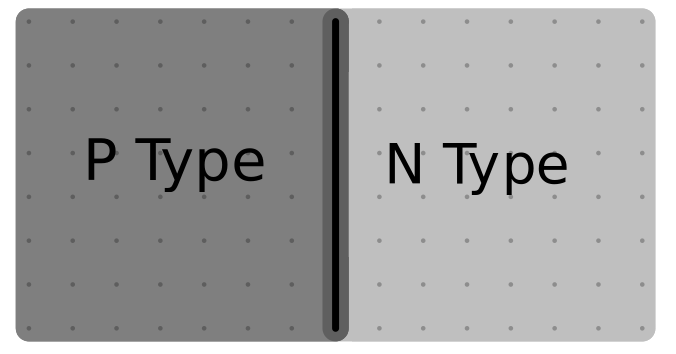
\includegraphics[width=0.23\linewidth]{pn-junction}
	\end{center}

	We have constants of $L_p$ and $L_n$ for the spacial exponential decay of the P or N charges. 
	
	Then the numbers $N_A$ and $N_D$ are porportional to the number of positive and negative charges respectively. They are the number of \textit{acceptor} or \textit{donor} atoms. 
	
	If $A$ is the area, then we say that the total diffusion current density is:
	\begin{align*}
		J_{diff\_tot} = Aqn_i^2\left(\frac{D_p}{L_pN_D}+\frac{D_n}{L_nN_A}\right)\left(e^{\frac{v}{V_t}}-1\right)
	\end{align*}
	This is also the total current since the drift current in a PN junction is small due to the generated electric field. 
	
	
	
	\section{Circuit Analysis with Diodes}
	We have three models for diodes. There is the ideal, constant voltage (ideal with voltage source), and constant voltage with resistance (ideal with voltage source and resistance). All of these model the real diode. 
	\begin{center}
		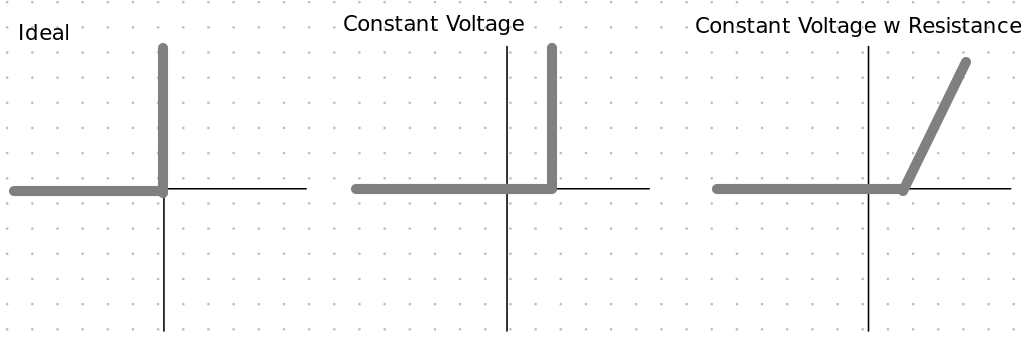
\includegraphics[width=0.8\linewidth]{diode-models}
	\end{center}

	An ideal diode can be either in the ON state (where current passes through in the correct direction) or the OFF state (where it acts as an open circuit). The other models just have this ideal diode with the voltage and resistance in series. 
	
	To determine the state of the diode, we need to assume a state (OFF or ON) and then check if it makes sense.
	\begin{itemize}[]
		\item If it is ON, then current MUST go from anode to cathode.
		\item If it is OFF, then voltage at cathode must be HIGHER than voltage at anode. 
	\end{itemize}

	If either of these criteria are wrong, then our assumption is on, and we need to try another one. 
	
	For reference, the diode looks like the following:
	\begin{center}
		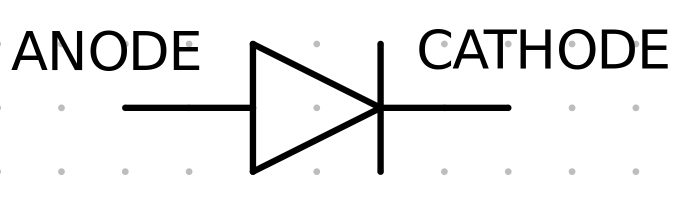
\includegraphics[width=0.3\linewidth]{diode-anode-cathode}
	\end{center}
	
	
	NOTE: There can only be \textbf{one } combination that works with a circuit. So if we have 2 diodes, and the first try it works, then it MUST be ONLY that combination.
	
	\begin{mdframed}[]
		\textbf{Ex. }In the following circuit, find $V_{out}$.
		\begin{center}
			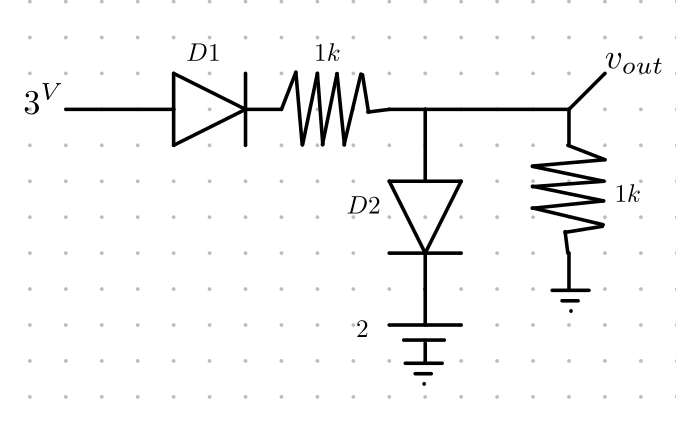
\includegraphics[width=0.4\linewidth]{diodes-ex}
		\end{center}
		We need to start by replacing the diodes with their model. I will use the ideal model for this example. So the diode is replaced by either a short circuit if ON, or an open circuit if OFF. 
		
		I will assume that $D1$ is OFF, and $D2$ is OFF. 
		\begin{center}
			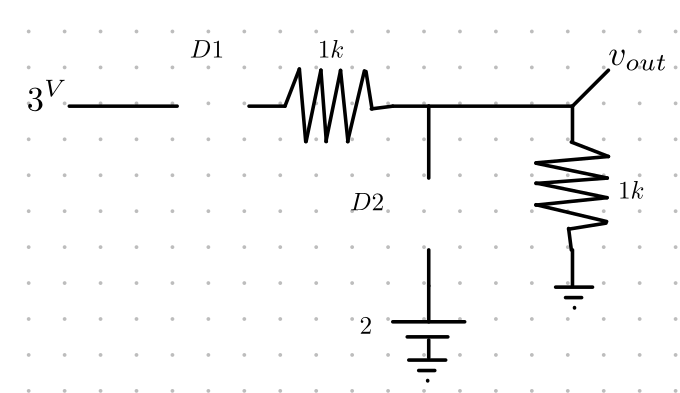
\includegraphics[width=0.4\linewidth]{diodes-ex1.1}
		\end{center}
		Now I need to check the conditions which for OFF is that the cathode voltage is greater than the anode voltage. 
		
		I see that the anode voltage is $3^V$, and the cathode voltage is $0^V$. So our assumption is WRONG.
		
		I will try another assumption of $D1$ is ON, $D2$ is OFF.
		\begin{center}
			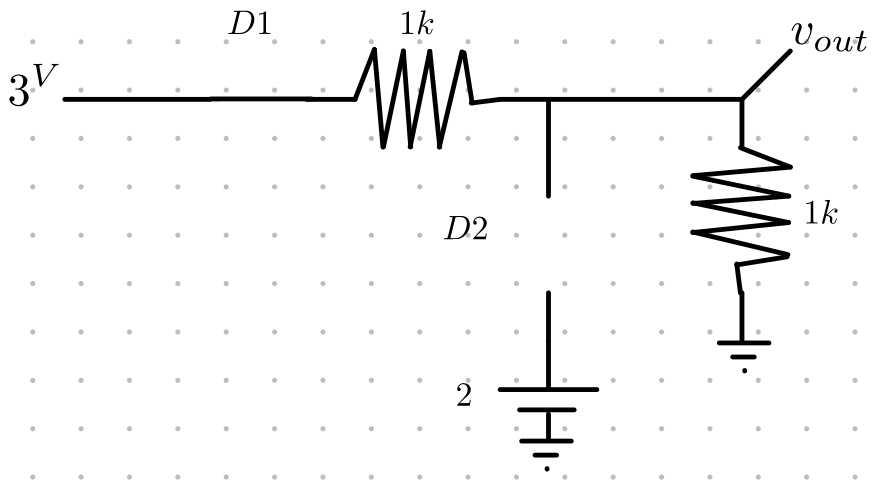
\includegraphics[width=0.4\linewidth]{diodes-ex1.2}
		\end{center}
		For $D1$ which is ON, I need to find the current and see that it is positive. I do a KVL starting at the 3V source, and going right. 
		\begin{align*}
			3 = 1k(I)+1k(I) \implies I=1.5mA \qquad \checkmark
		\end{align*}
		Now for $D2$ I need to check that the cathode voltage is greater than anode voltage. Using a voltage dividor, the anode voltage is 1.5V, then from observation the cathode voltage is 2V. $\checkmark$
		
		Now we know that this is the state of the circuit. We DO NOT need to check any other situations since there can ONLY be ONE correct configuration. 
		
		Now we can analyse and find that $V_{out} = 1.5^V$
		
	\end{mdframed}

	\begin{mdframed}
		\textbf{Ex.} For the previous example, find $V_{out}$ using the constant voltage model.
		
		Here we just need to modify the diagram to add a 0.7V source to each diode. I will test out $D1$ is ON and $D2$ is OFF.
		\begin{center}
			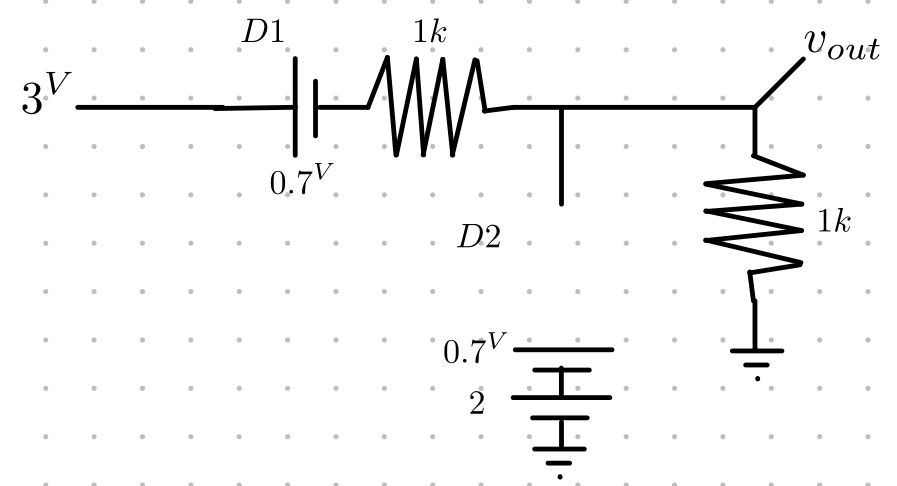
\includegraphics[width=0.4\linewidth]{diodes-ex2.1}
		\end{center}
		For the ON diode, I find that the current is 1.15mA through a KVL. 
		
		For the OFF diode I find that the anode (top) is 1.15V, and the cathode (bottom) is 2.7V. 
		
		Note that I consider this as the voltage drop over the ideal diode component of the constant voltage model, not the entire diode. 
		
		Now I find $V_{out} = 1.15V$.
	\end{mdframed}
	
	\subsection{Plotting}
	For these problems, we have a circuit, and we have an input voltage (x axis) and another value such as output voltage, or output current, and we need to \textbf{plot the output as a function of the inputs}. 
	
	This is a lot of work since we have diodes, and when each diode changes, as will the relation between the input and the output. 
	
	This is the procedure: 
	\begin{enumerate}[noitemsep]
		\item Replace all diodes with their model (Ideal, Constant Voltage, CV with Resistance)
		\item Assume very low value for X (input) and find the state of each diode using this low value.
		\item Analyse the circuit to find Y (output) as a function of X (input)
		\item Find out which diode will switch its state \textbf{first }(let ON diode current=0, or OFF diode voltage=0)
		\item Replace the diode whose state changes first with its new state and \textit{return to step 3}. 
		\item STOP analysis once no more diodes will change state (diodes only change states at most 1 time).
	\end{enumerate}

	\begin{mdframed}[]
	\textbf{Ex. }Find $V_{out}$ as a function of $V_{in}$ using ideal diode model.
	\begin{center}
		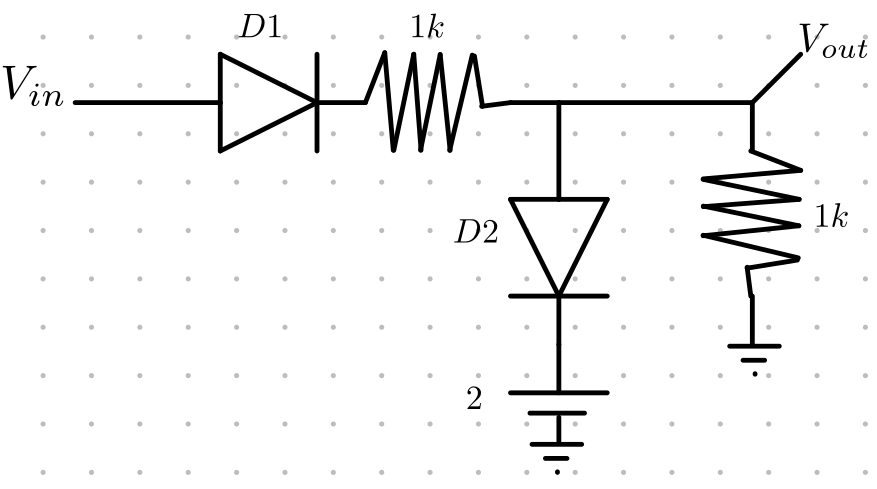
\includegraphics[width=0.4\linewidth]{diodes-plotting-1.1}
	\end{center}
	First I need to find the state when $V_{in}$ is very small ($-\infty$).
	
	If the input is very small, then D1 must be off since by definition $V_{in}$ is the smallest voltage in the circuit, so the other side must be larger. 
	
	This creates an open circuit over D1 causing the rest of the loop to be a simple KVL. We find that D2 must also be OFF. 
	\begin{center}
		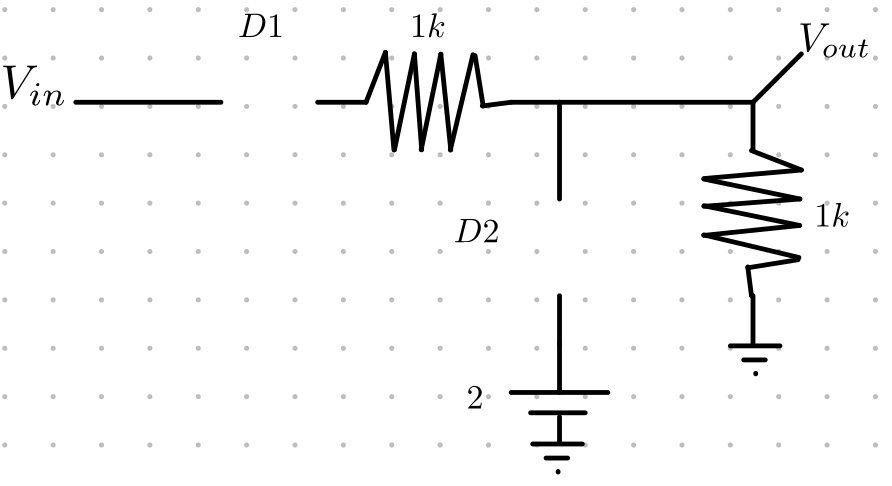
\includegraphics[width=0.4\linewidth]{diodes-plotting-1.2}
	\end{center}
	We can see that for this interval, \textbf{the output is 0V.}
	\begin{center}
		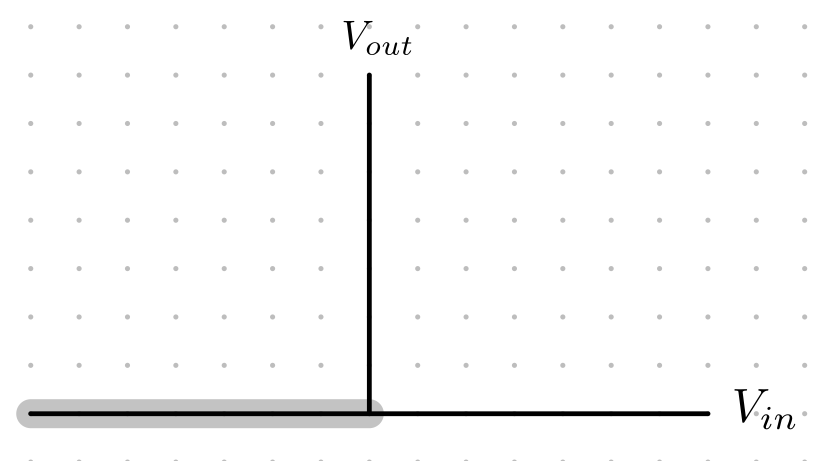
\includegraphics[width=0.3\linewidth]{diodes-plotting-1.3}
	\end{center}
	Now we need to find when one of the diodes will change states. This is when the voltage across one of the diodes becomes 0. Here it must be a value of $V_{in}$ that causes this change. 
	\begin{align*}
		D1: V_{in} &= V_{D1} + 1k(I) + V_{out}&\\
			&=0 + 0 & \text{No current $I$, and $V_{D1}$ is 0}\\
			&= V_{out} = 0 &\text{Since we know $V_{out}=0$}\\
		D2: V_{out} &= V_{D2} + 2&\text{KVL starting with $V_{out}$}\\
			\implies 0 &= 2 \qquad X &\text{Since we know $V_{out}=0$}
	\end{align*}
	So D1 must change first. Now I change D1 to ON to get:
	\begin{center}
		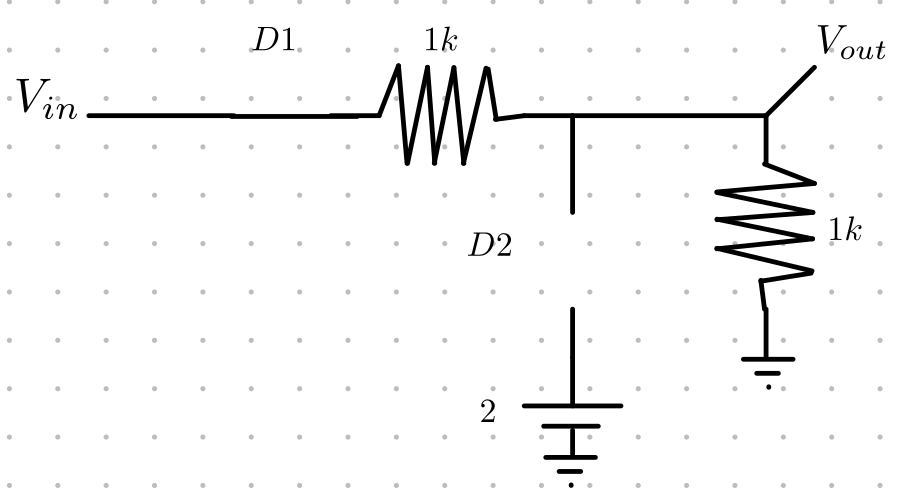
\includegraphics[width=0.4\linewidth]{diodes-plotting-1.4}
	\end{center}
	We need to find $V_{out}$ as a function of $V_{in}$ for this part as well. 
	\begin{align*}
		&V_{out} = \frac{V_{in}}{2}&\text{I see this from the circuit} \\
		&&\text{It can also be found from voltage dividor}
	\end{align*}
	\begin{center}
		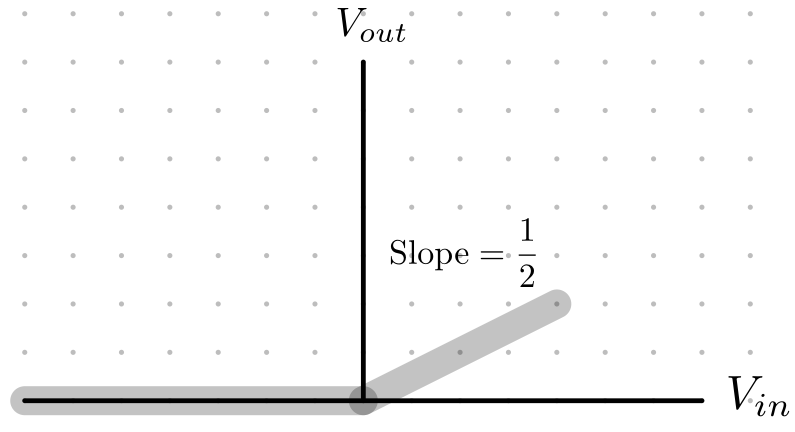
\includegraphics[width=0.3\linewidth]{diodes-plotting-1.5}
	\end{center}
	Now I need to find the last break point (if it exists). This will be when D2 changes since D1 cannot change again. This can be either the value of the \textit{input or output} since both are changing. 
	\begin{align*}
		V_{out} = V_{D2} + 2 = 2 \implies V_{in} = 2V_{out} = 4
	\end{align*}
	So D2 will change to ON when the input is 2, and the output is 4. 
	
	Finally we need to know what the ouput actually changes to when this happens.
	\begin{center}
		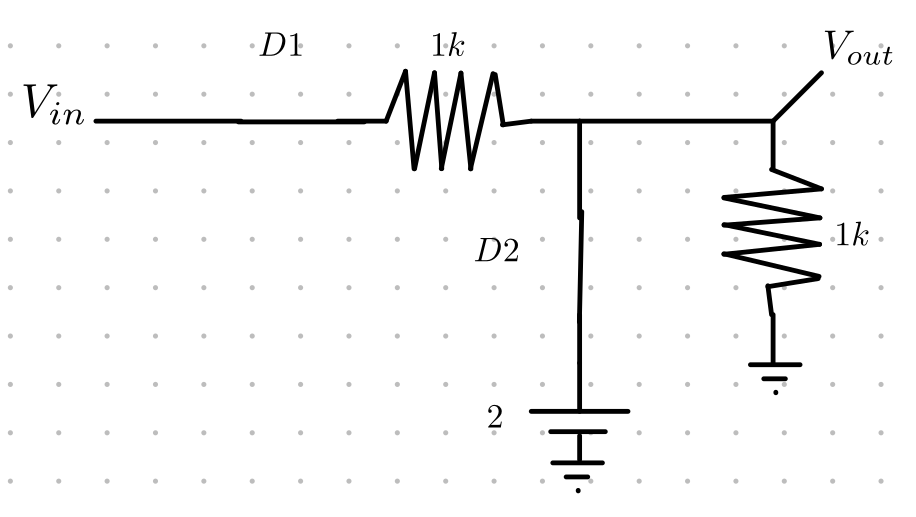
\includegraphics[width=0.4\linewidth]{diodes-plotting-1.6}
	\end{center}
	We can see that the output is just parallel with the constant 2V source. So it is just 2 Volts. 
	\begin{center}
		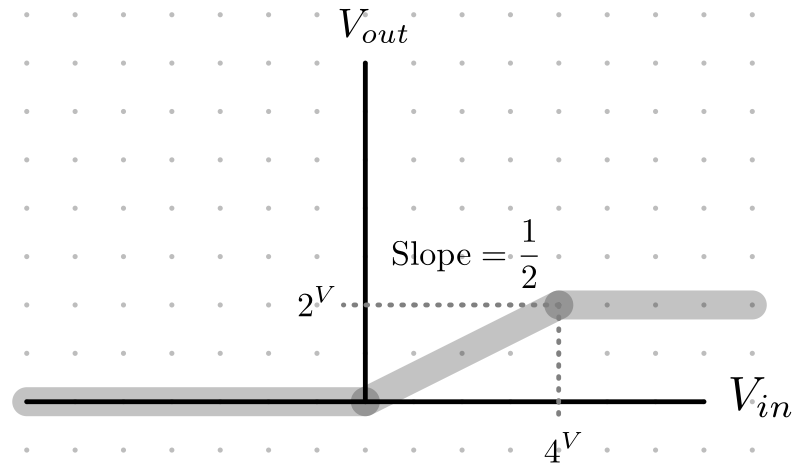
\includegraphics[width=0.5\linewidth]{diodes-plotting-1.7}
	\end{center}
	
	\end{mdframed}
	
	\section{DC Power Supply}
	This is a very important application of diodes. This will convert an AC time dependant source to a DC constant source. 
	
	\subsection{Rectifier}
	The rectifier will take an AC source, and make the output be positive.
	\begin{center}
		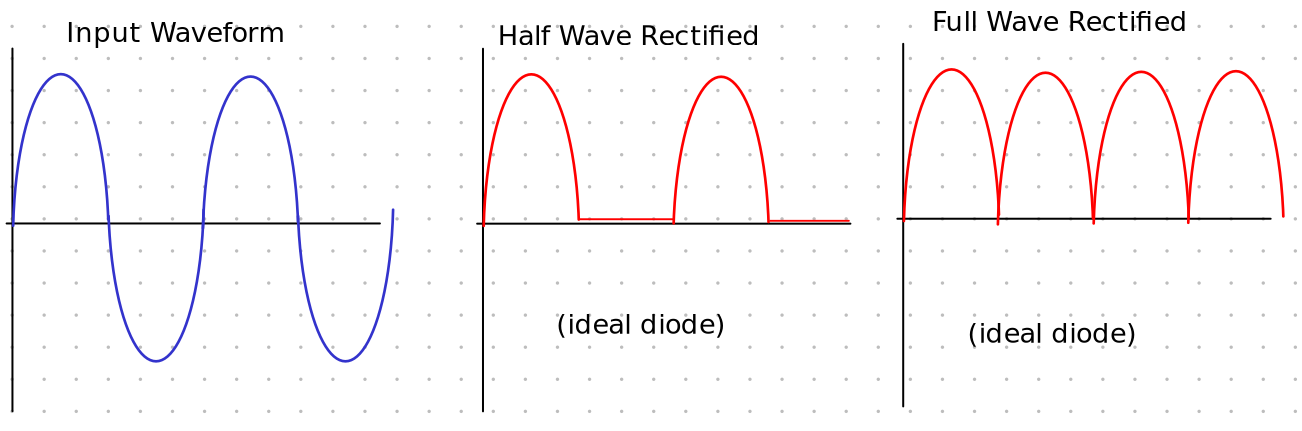
\includegraphics[width=0.9\linewidth]{rectifier}
	\end{center}
	
	
	A Half wave rectifier (1 diode) will just kill the negative part of the wave, while a Full wave rectifier (2 diodes) will keep the positive part, and invert the negative part. 
	
	A Bridge rectifier is a special type of full wave rectifier that has 4 diodes instead of 2. 
	
	A useful statistic is the PIV (Peak Inverse Voltage) across a diode. To find this, we take a diode that we want to find the PIV across, then we find what would be the maximum negative voltage across this diode (note the diode will be OFF) when the source is at its inverse peak. 
	
	Typically we do a KVL through the circuit. Note that we find the voltage across the whole diode (including voltage and resistance if using that model).
	
	
	\subsection{Filter}
	The Filter is just adding a capacitor in parallel with the load resistor. This will \textbf{smooth out the big inflections}, but there will still be a ripple. 
	\begin{center}
		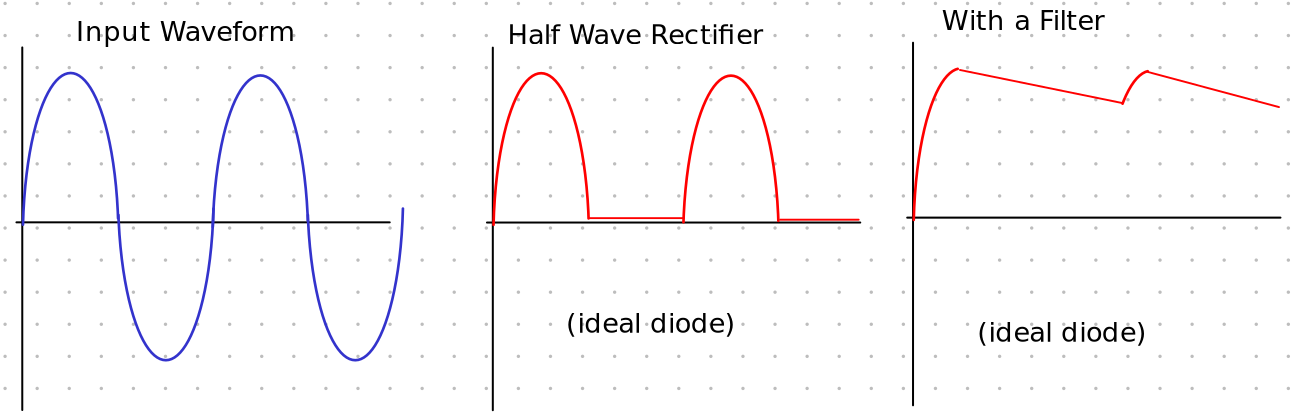
\includegraphics[width=0.9\linewidth]{filter}
	\end{center}

	We call $V_p$ the peak voltage of the wave, $V_r$ as the ripple voltage (if it fluctuates between 9 and 11 V, then $V_4=2V$), and $V_k$ as the minimum voltage.
	\begin{align*}
		V_p = V_k + V_r
	\end{align*}
	We can make some approxmiations (with ideal diodes) to see that:
	\begin{align*}
		V_r &= \frac{V_p}{fRC} \text{ for a half wave rectifier or } \\
		V_r &= \frac{V_p}{2fRC} \text{ for a full wave }\\
		\omega\Delta t &= \sqrt{\frac{2V_r}{V_p}} \text{ for both types of rectifiers}\\
		\text{Current through diode average }i_{Davg} &= I_L(1+\pi\sqrt{\frac{2V_p}{V_r}}) \text { for half wave} \\ 
		\text{or for full wave } i_{Davg} &= I_L (1+\pi\sqrt{\frac{V_p}{2V_r}}) \\
		\text{Current through diode MAX }i_{Dmax} &= I_L(1+2\pi\sqrt{\frac{2V_p}{V_r}}) \text{ for half wave }\\ 
		\text { or for full wave } i_{Dmax} &= I_L (1+2\pi\sqrt{\frac{V_p}{2V_r}}) \\
	\end{align*}

	If we are working with a different model, such as the constant voltage model, then we will need to modify the equations such as increasing the peak voltage by 0.7V. The one exception is the conduction angle formula $\omega \Delta t$ since that is not affected by te extra 0.7V.
	
	For most of the equations, we use the peak voltage at the source. The only exception is the capacitor formula where we use the peak voltage at the capacitor. 
	
	\begin{mdframed}[]
		\textbf{Ex. }We have a bridge rectifier with a filter capacitor as shown below. We want to find the PIV if the filter is disconnected, or connected. Then we want to find the capacitence required for a ripple of 2V. We also want to conduction angle (with the filter connected).
		\begin{center}
			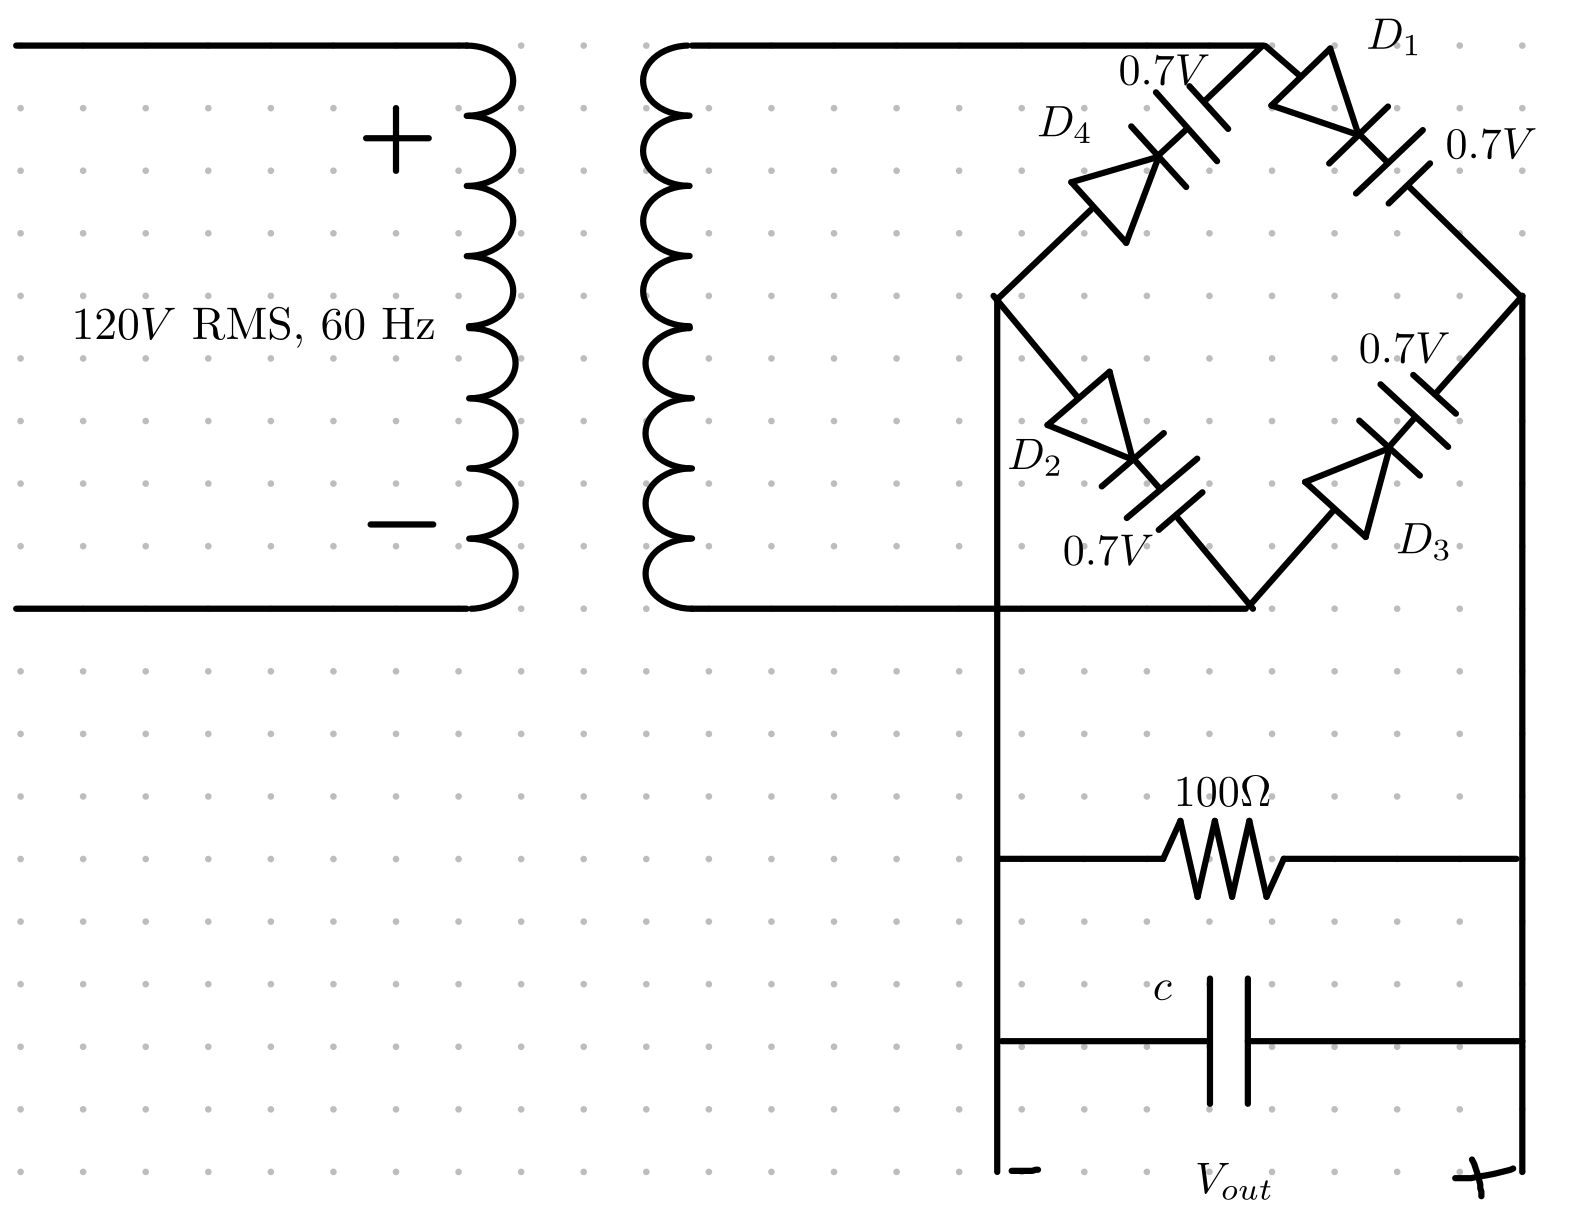
\includegraphics[width=0.7\linewidth]{filter-ex}
		\end{center}
		First we need to find the peak voltage on the secondary side of the transformer. This needs to be high enough to overcome the two voltage drops from the diodes, and must be 1V higher than needed for the ripple:
		\begin{align*}
			V_s = 0.7+0.7+10+1=12.4V
		\end{align*}
	
		If the filter is disconnected, the PIV can be found taking a KVL through the circuit starting at the source in the reverse direction (not going through the capacitor since this is disconnected):
		\begin{align*}
			-12.4 + 0 + 0.7 = -11.7V \implies PIV = 11.7
		\end{align*}
		\begin{center}
			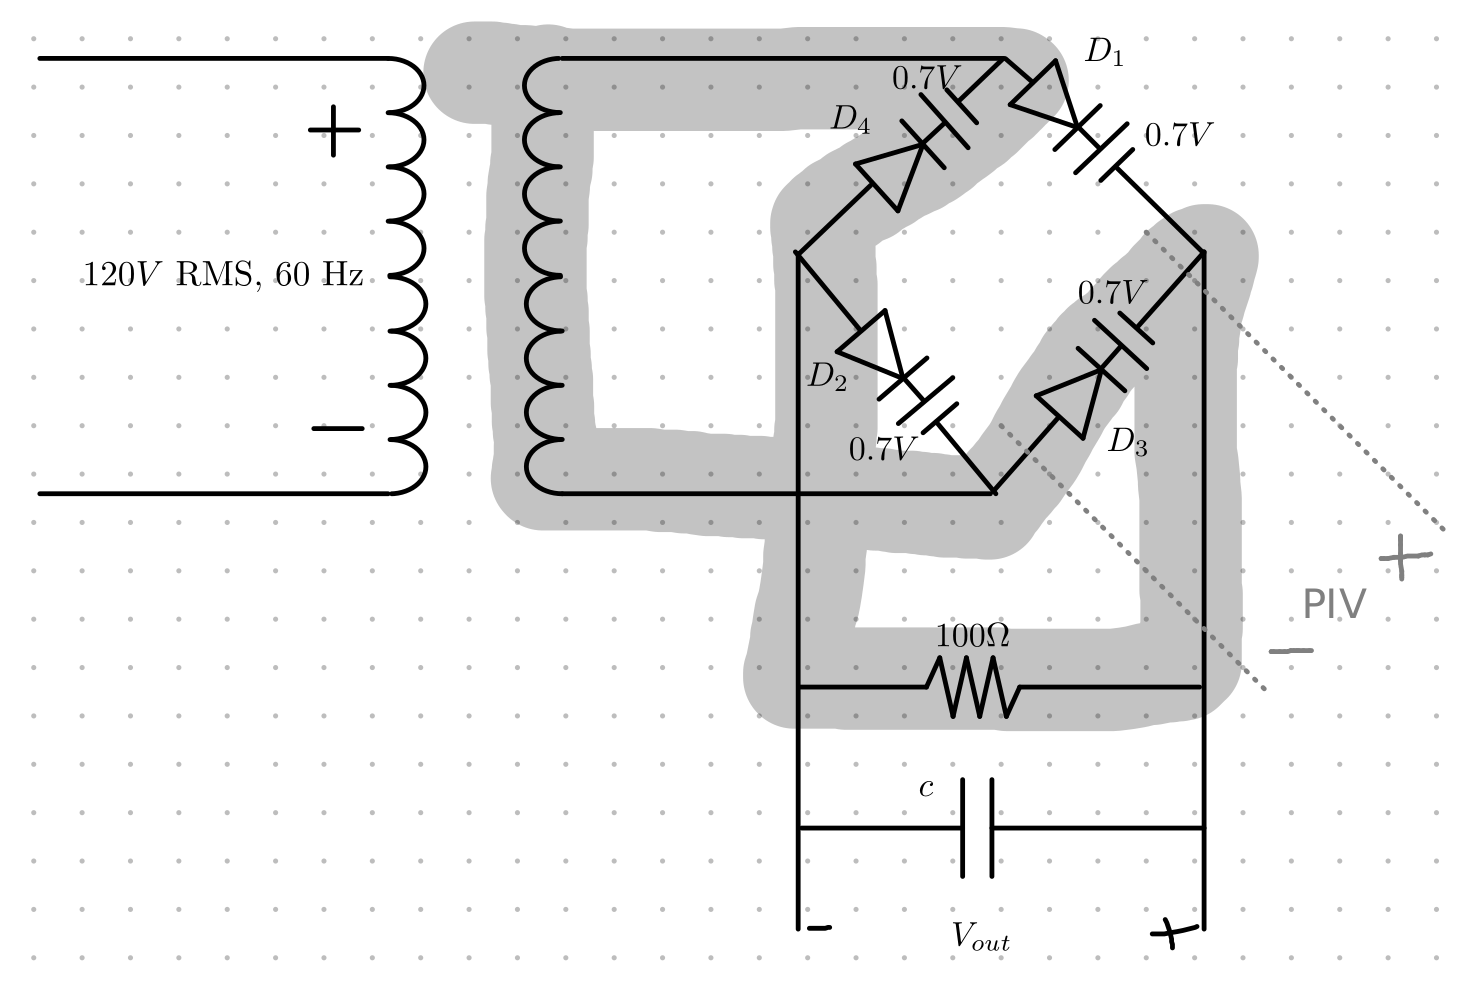
\includegraphics[width=0.5\linewidth]{filter-ex1}
		\end{center}
	
		If the filter is connected, we will take a KVL through a similar loop, except we go through the capacitor since it gives 10V average voltage. 
		\begin{align*}
			-12.4+0+0.7-10=-21.7V \implies PIV = 21.7
		\end{align*}
		The waveforms generated will be as follows:
		\begin{center}
			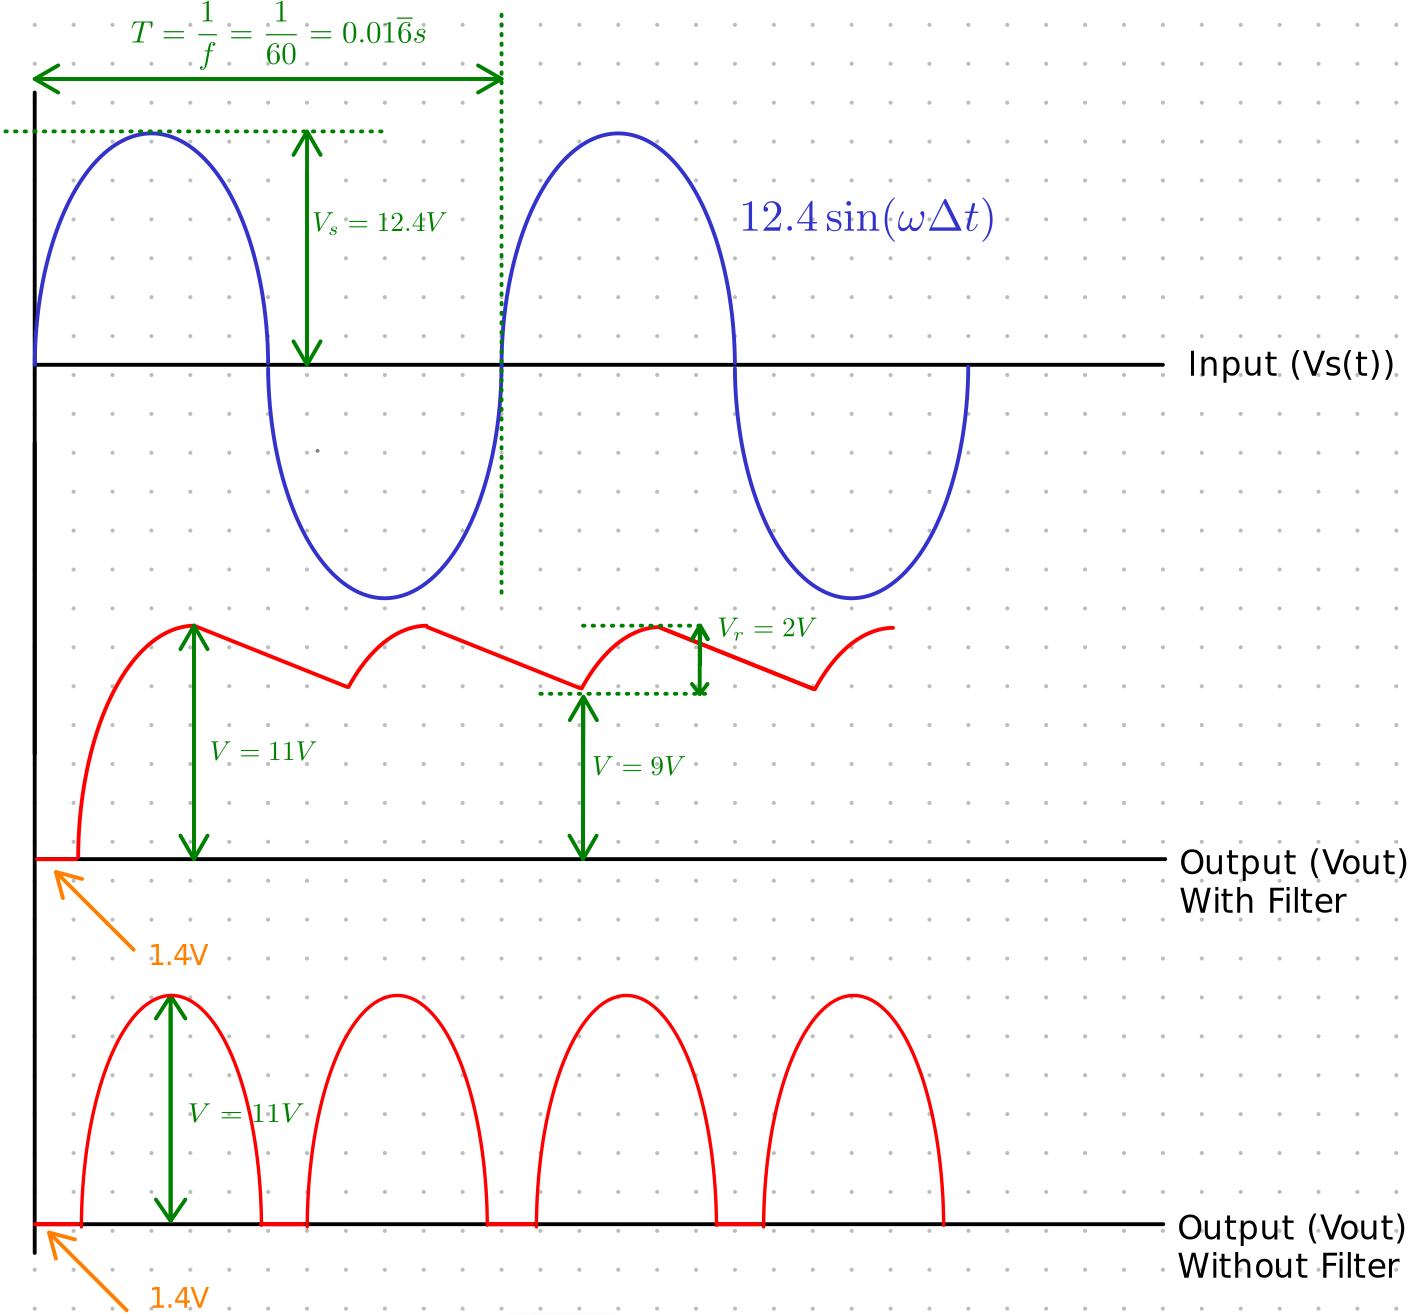
\includegraphics[width=0.7\linewidth]{filter-ex2}
		\end{center}
		Finding the capacitence is simple. We know that the peak voltage through the capacitor is 11V, and we know the frequency, ripple, and load resistance. So we use the formula:
		\begin{align*}
			V_r = \frac{V_p}{2fRC}\implies C = \frac{V_p}{2V_rfR} = \frac{11}{2\cdot 2\cdot 60\cdot 100} = CALC
		\end{align*}
		Same idea for the conduction angle except for that works off the peak voltage at the source. 
		\begin{align*}
			\omega\Delta t = \sqrt{\frac{2V_r}{V_p}} = \sqrt{\frac{2\cdot 2}{12.4}} = CALC
		\end{align*}
		
	\end{mdframed}
	
	\subsection{Regulator}
	The regulator is a function that takes in a voltage source with unwanted ripples, and greatly \textbf{reduces these ripples}. It does this with a diode working in the breakdown region (zener diode).
	\begin{center}
		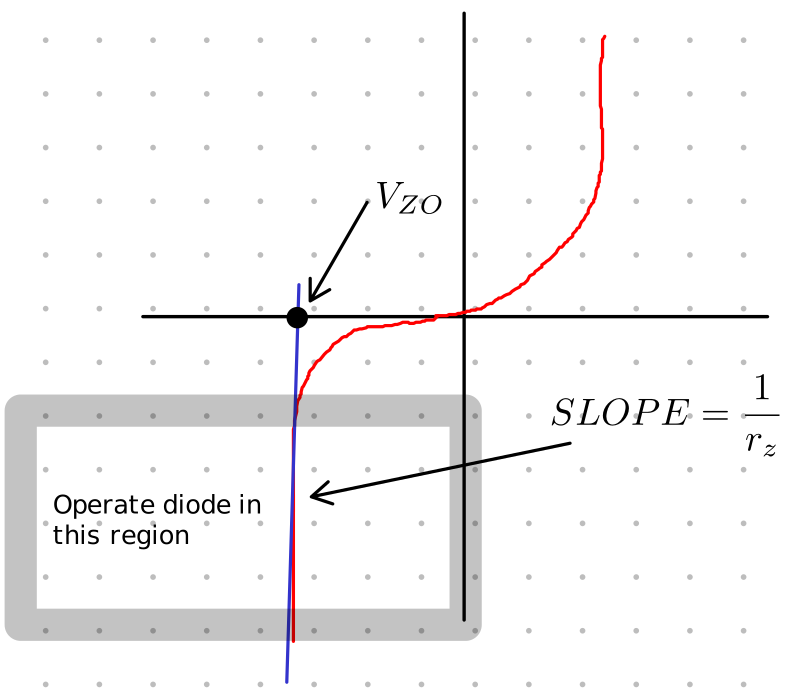
\includegraphics[width=0.4\linewidth]{regulator}
	\end{center}
	$r_z$ is the internal resistance of the diode. $V_{ZO}$ is the internal voltage source of the diode. 
	
	We need to ensure that the zener operates \textbf{only in the breakdown region} for no fluctuations in the output voltage. We do this by finding the minimum and maximum current allowed for the diode to stay in the breakdown region (straight line part).
	
	We want to maintain the output voltage to be as constant as possible, and this is measured using the line and load regulation. 
	\begin{align*}
		\text{Line Regulation}=\frac{\Delta V_O}{\Delta V_s} = \frac{r_z}{r_z+R} \qquad \text{Load Regulation}=\frac{\Delta V_O}{\Delta I_L} = -\frac{r_z\times R}{r_z+R} = -r_z // R
	\end{align*}

	\begin{mdframed}[]
		\textbf{Ex. }We have a zener regulator. We have two datapoints. When $V_Z=10.1V$, $I_Z = 0.01A$. When $V_Z=10.2V$, $I_Z=0.02A$. Find the zener diode resistance and voltage $r_z, V_{ZO}$. 
		\begin{center}
			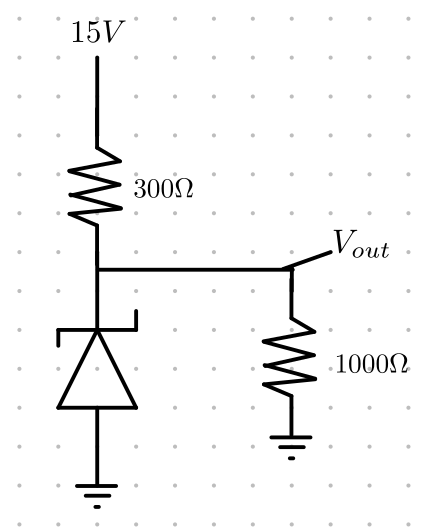
\includegraphics[width=0.33\linewidth]{zener}
		\end{center}
		To find the zener resistance, we use the standard slope equation:
		\begin{align*}
			SLOPE = \frac{\Delta i}{\Delta V} = \frac{0.02-0.01}{10.2-10.1}=0.1
		\end{align*}
		Since the zener resistance is the recipricol of the slope, $r_z = 10\Omega$.
		
		To find the voltage source, I will create an equation for the slope of the line, and then let the current equal 0 (current is $y$, voltage is $x$). 
		\begin{align*}
			&i = \frac{1}{r_z}V+c \implies 0.01 = \frac{10.1}{10} + c \implies c  = -1\\
			&0 = \frac{1}{10}V_{zo}-1 \implies V_{zo}=10
		\end{align*}
		Now we can go back to the circuit and replace the zener diode with its model of the voltage source and resistance.
		
		Note that since it is a zener diode, the voltage source is \textit{reversed}.
		\begin{center}
			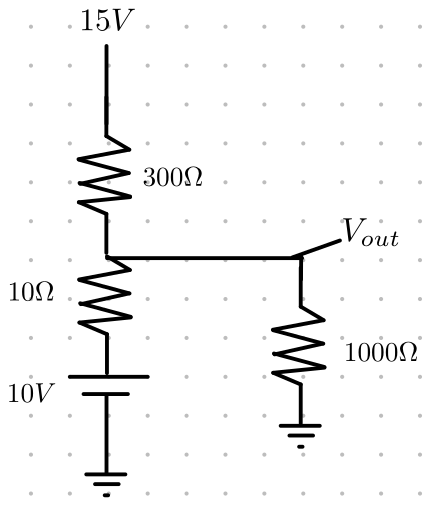
\includegraphics[width=0.33\linewidth]{zener1}
		\end{center}
		If we now want to find the output voltage, we can use any circuit analysis method such as source transformations to do:
		\begin{center}
			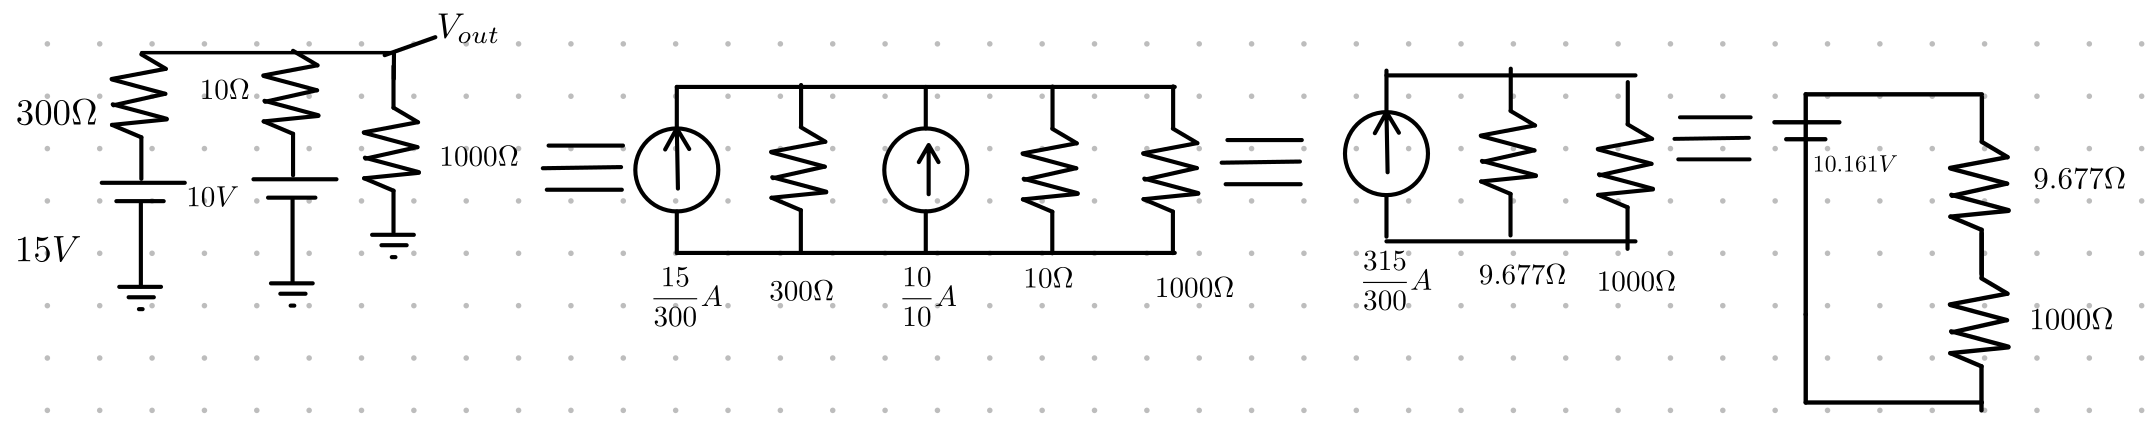
\includegraphics[width=1\linewidth]{zener2}
		\end{center}
		Then using a voltage dividor we can get the voltage. 
	
	\end{mdframed}
	
	\section{Bipolar Junction Transistor (BJT)}
	A BJT transistor has 2 PN junctions. 
	
	The BJT can either have P type sandwiched between 2 N types (NPN), or N type sandwiched between 2 P types (PNP). 
	\begin{center}
		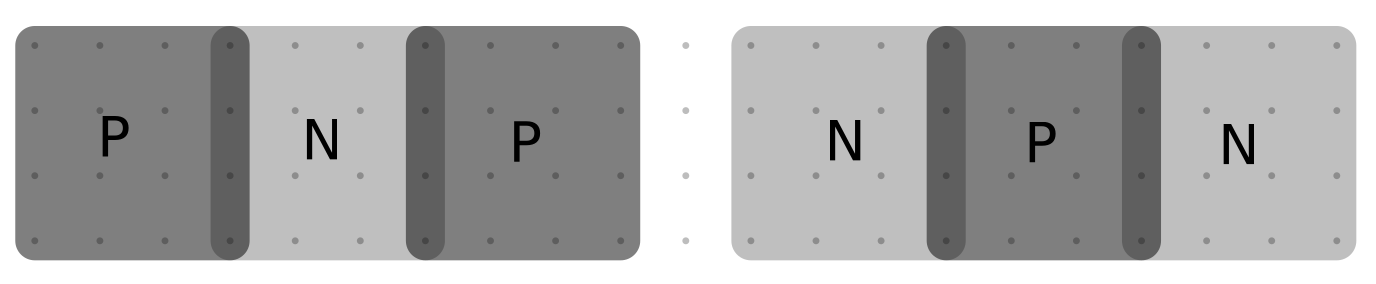
\includegraphics[width=0.7\linewidth]{pnp-vs-npn}
	\end{center}
	A BJT has three terminals called the \textbf{Emitter, Collector, and Base}. Each of these terminals needs to have a DC voltage applied. Depending on how these voltages relate to each other (biassing of each PN junction) makes the transistor operate differently. 
	
	In this course we only care about the \textbf{active} mode which is where for PNP, the emitter is the largest, followed by base, followed by collector, and for NPN, collector is largest, followed by base, followed by emitter. 
	
	In all cases, the BE junction has a difference of 0.7 volts due to the diode. 
	\begin{figure}
		\centering
		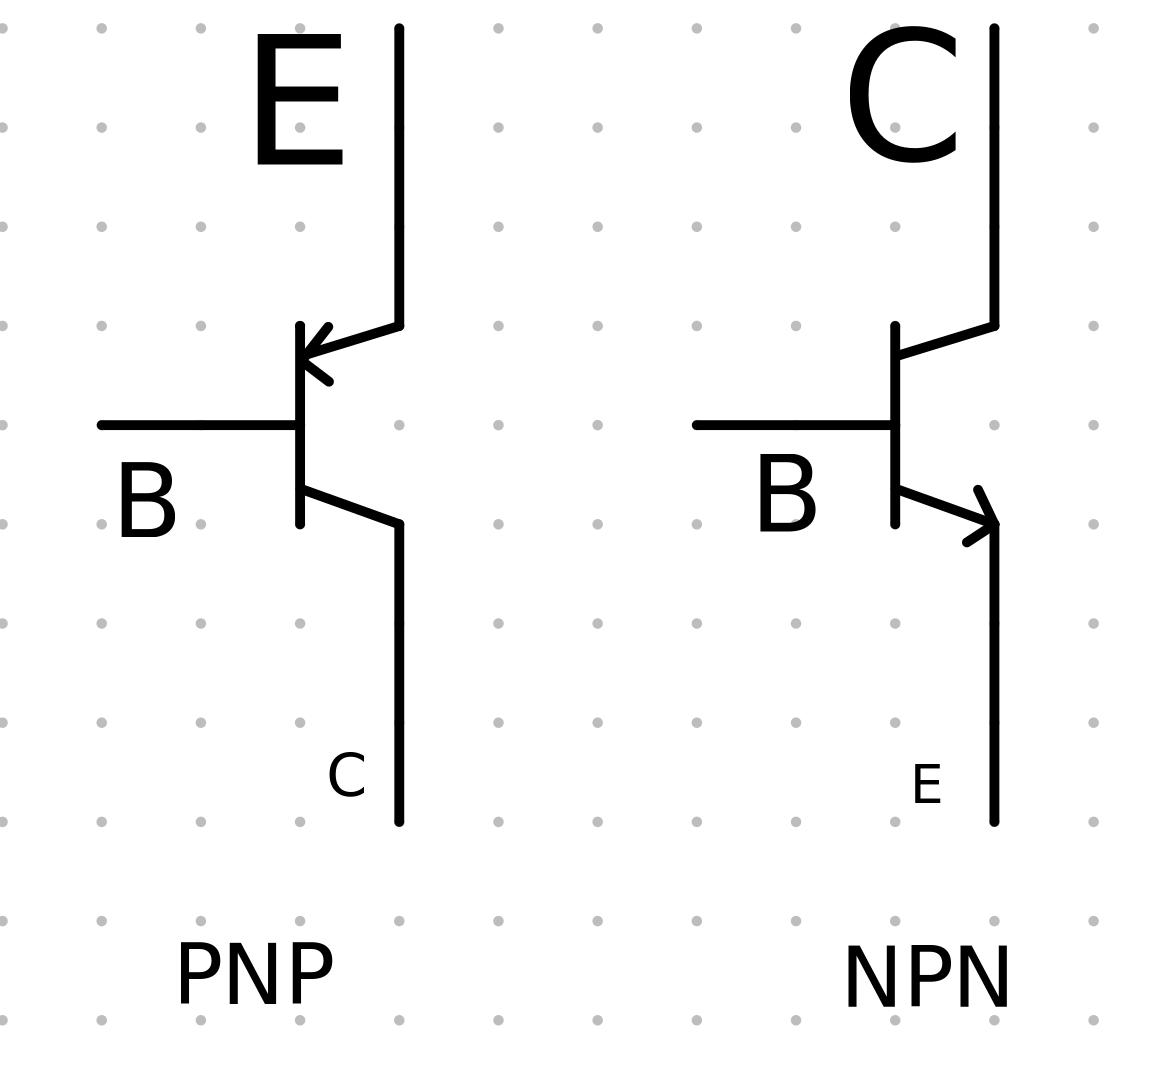
\includegraphics[width=0.4\linewidth]{bjt-biassing}
		\caption{Active Mode Bias}
		\label{figure:bjt-active-mode-bias}
		
	\end{figure}
	
	Going back to the PNP or NPN model, if the current flows from P to N, we say that junction is in forward bias. While if the current flows from N to P, we say that junction is in reverse bias. 
	\begin{center}
		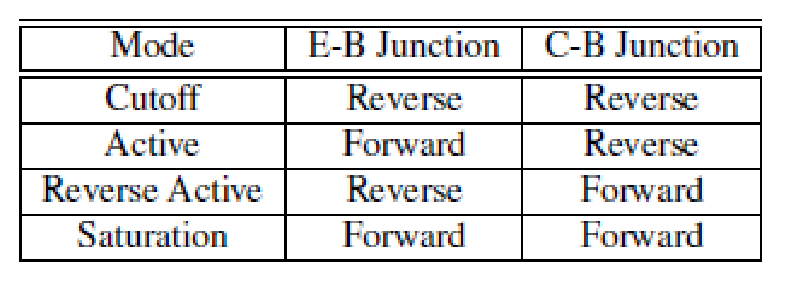
\includegraphics[width=0.5\linewidth]{bjt-bias-table}
	\end{center}
	
	\subsection{DC Analysis}
	To do the DC analysis, we need to figure out what mode the transistor is in. Typically for this course it is either in Cutoff mode (no current), or active mode (see Figure \ref{figure:bjt-active-mode-bias}).
	
	So we \textbf{assume active mode}, and see if there is a contradiction (such as negative or 0 current).
	
	We have some very useful relations for the currents which are:
	\begin{align*}
		&I_E = I_B + I_C & I_C = \beta I_B
	\end{align*}
	$\beta$ is a parameter of the specific BJT given in the \textbf{datasheet}.
	
	\subsection{AC Analysis}
	We need to introduce a new notation for this. We say that lowercase means ac, and uppercase means DC. Mixed case means a mixed signal.
	\begin{align*}
		&v_A& \text{ac and DC Signal}\\
		&v_a &\text{Pure ac Signal}\\
		&V_A &\text{Pure DC signal}
	\end{align*}

	To get the current, \textit{sometimes} we are given the $I_S$ parameter. This gives:
	\begin{align*}
		i_C = I_S e^{\frac{v_{BE}}{V_T}} \text{ for NPN or replace $V_{BE}$ with $V_{EB}$ for PNP}
	\end{align*}
	Here $V_T$ is a known value that is given on the \textbf{datasheet}. 
	
	With ac analysis, we generally do not know the ac currents or voltages since these fluxuate with time. But we do know the resistances and the DC currents. Through this information we can get the following parameters:
	\begin{align*}
		g_m = \frac{I_C}{V_T} \qquad r_\pi  =\frac{\beta}{g_m} = \frac{V_T}{I_B} \qquad r_e = \frac{\alpha}{g_m}\qquad \alpha = \frac{\beta}{\beta+1}
	\end{align*}
	\textbf{NOTE that $V_T$ is a constant with value 25mV}
	
	Then we also have other parameters that we need to find through circuit analysis such as KVL or KCL. These are things such as:
	\begin{align*}
		&A_V = \frac{v_{out}}{v_{in}}&\text{Voltage Gain}\\
		&G_v = \frac{v_{out}}{v_{sig}}&\text{Overall Voltage Gain}\\
		&A_i = \frac{i_{out}}{i_{in}}&\text{Current Gain}\\
		&R_{in} &\text{Input Resistance}\\
		&R_{out}&\text{Output Resistance} 
	\end{align*}
	When doing these, the answer \textbf{MUST NOT be in terms of time dependant values} such as ac current, or ac voltage.
	
	To do this, we need to change the BJT transistor for a \textbf{model}. We have the Hybrid Pi model, or the T model. 
	\begin{center}
		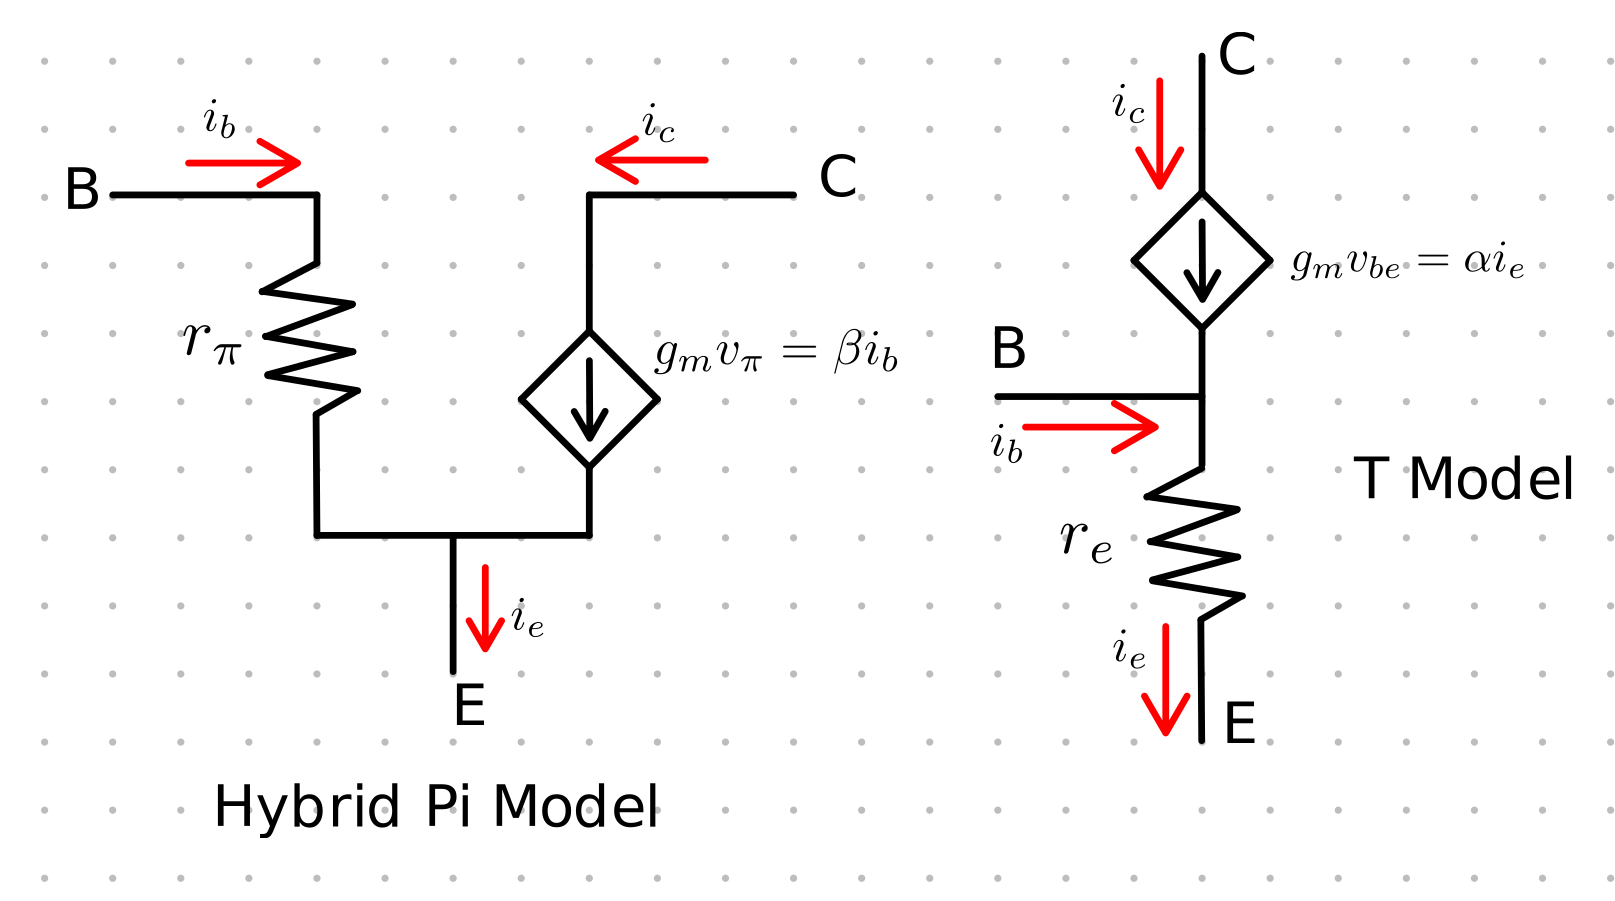
\includegraphics[width=0.8\linewidth]{hybridpi-tmodel}
	\end{center}
	
	\subsection{ac and DC Analysis Combined}
	When combining the two analyses, we can consider each one individually and follow the following technique:
	\begin{itemize}
		\item DC Analysis
		\subitem Short Circuit all ac voltage sources and Open Circuit all ac current sources
		\subitem Short circuit all inductors, and open circuit all capacitors
		\subitem Find C, B, E currents and voltages, find $g_m$, and confirm it is in active mode.
		\item ac Analysis
		\subitem Short Circuit all DC voltage sources and Open Circuit all DC current sources
		\subitem Short circuit all capacitors, and open circuit all inductors
		\subitem Solve for what we want (such as $A_V$ or $R_{in}$)
	\end{itemize}

	\begin{mdframed}
		\textbf{Ex. }Using the below circuit, find the voltage gain, the input resistance, and the output resistance. We know that $\beta = 100$
		\begin{center}
			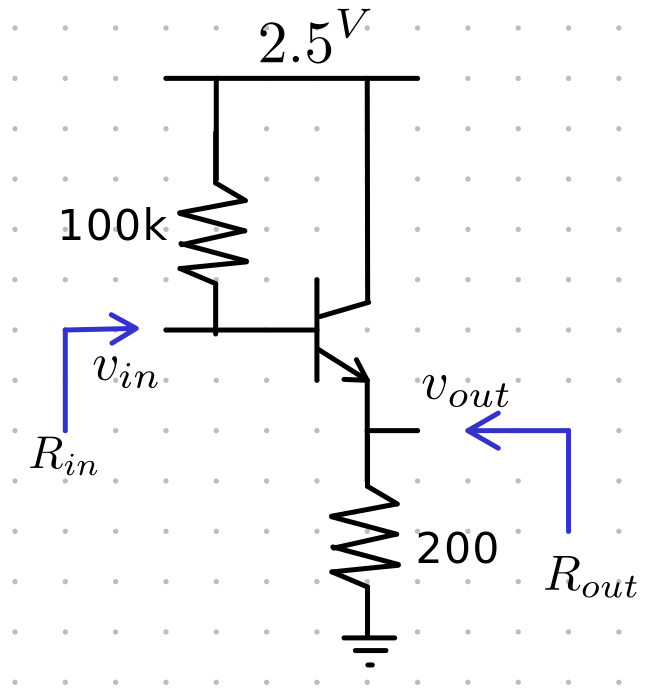
\includegraphics[width=0.3\linewidth]{bjt-ex}
		\end{center}
		First we need to do the\textbf{ DC analysis}. The first step is always to do a KVL through the BE part since we know the voltage drop is 0.7 Volts. We also have to disable the ac sources. I can also label the Collector, Base, and Emitter using the NPN values since arrow going out of the BJT.
		\begin{center}
			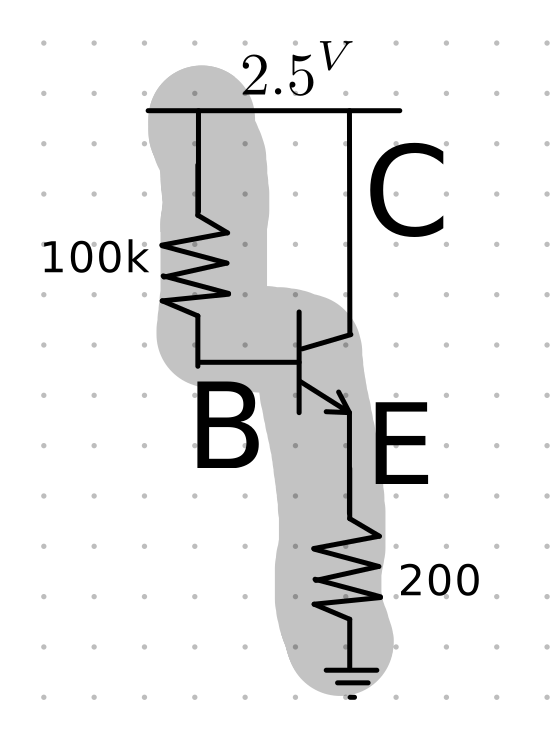
\includegraphics[width=0.1\linewidth]{bjt-ex1}
		\end{center}
		\begin{align*}
			2.5-100000I_B - 0.7 - 200 I_E= 0
		\end{align*}
		Now using the relation between the three currents, we can get that $I_E = I_C + I_B = I_B (\beta + 1)$
		\begin{align*}
			2.5-100000I_B - 0.7 - 200 (101) I_B= 0 \implies I_B = 1.498 \mu A \implies I_C = 1.498 mA
		\end{align*}
		To ensure the BJT is in active mode, I find the voltages at all three places:
		\begin{align*}
			&V_C = 2.5^V\qquad V_B = 2.5-100000I_B = 1.002^V \qquad V_E = 1.002-0.7 = 0.3\\
			& V_C > V_B > B_E \qquad \checkmark
		\end{align*}
		Now we move to \textbf{ac analysis} starting with finding the circuit parameters.
		\begin{align*}
			&g_m = \frac{I_C}{V_T} = \frac{1.498}{25}=0.05992 &r_\pi = \frac{\beta}{g_m} = 1669
		\end{align*}
		Now we can set up the ac circuit by disabling DC sources and using an ac model. I will use the Hybrid Pi model. 
		\begin{center}
			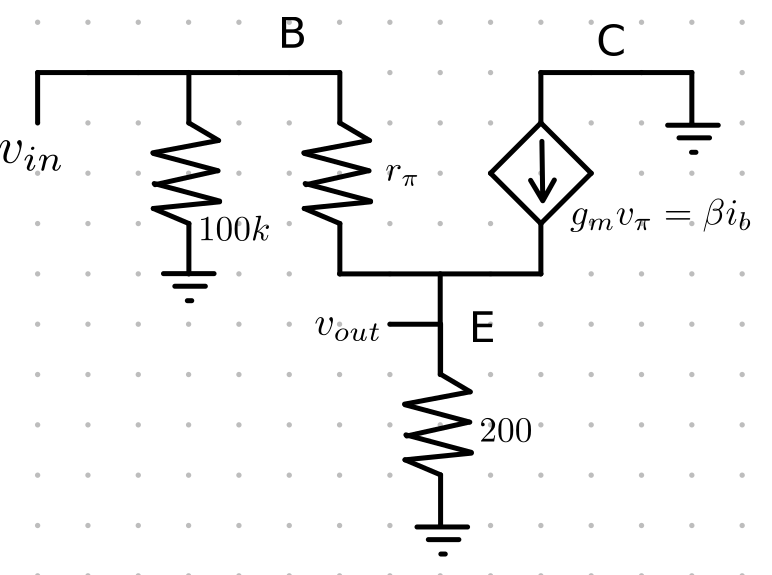
\includegraphics[width=0.4\linewidth]{bjt-ex2}
		\end{center}
		To find the \textbf{Voltage gain} $A_V = \frac{v_o}{v_i}$, we can create some KVLs.
		\begin{align*}
			&v_{in} = v_\pi + 200i_E = i_B r_\pi + 200i_E\\
			&v_{out} = 200i_E\\
			&A_V = \frac{v_o}{v_i} = \frac{200i_E}{i_Br_\pi+200i_E}
		\end{align*}
		Well this is a problem since we cannot have \textbf{any time dependant currents/voltages}. But if we write $i_B$ in terms of $i_E$, we can cancel out all $i_E$ to get no time dependant sources.
		\begin{align*}
			&A_V = \frac{v_o}{v_i} = \frac{200i_E}{\frac{i_E}{\beta +1}r_\pi+200(i_E)} = \frac{200}{\frac{r_\pi}{\beta +1}+200} = 0.92
		\end{align*}
		To find the \textbf{input resistance}, we can create a test source at $R_{in}$, disable all INDEPENDANT sources, and then solve for $\frac{V_{test}}{I_{test}}$. 
		
		In this case, we already have a source ($V_{in}$) so we do not need to create a test source. We just need to find the input current. 
		\begin{align*}
			&v_{in} = \frac{i_E}{\beta +1}r_\pi+200(i_E)\\
			&i_{in} = i_{100k} + i_b = \frac{v_{in}}{100k} + \frac{i_E}{\beta + 1} = \frac{\frac{i_E}{\beta +1}r_\pi+200(i_E)}{100k} + \frac{i_E}{\beta + 1}\\
			&R_{in} = \frac{v_{in}}{i_{in}} = \frac{\frac{i_E}{\beta +1}r_\pi+200(i_E)}{\frac{\frac{i_E}{\beta +1}r_\pi+200(i_E)}{100k} + \frac{i_E}{\beta + 1}} = \frac{\frac{1}{\beta +1}r_\pi+200}{\frac{\frac{1}{\beta +1}r_\pi+200}{100k} + \frac{1}{\beta + 1}} = 17.95k
		\end{align*}
		To find the \textbf{output resistance} we follow a similar procedure except for we need a test source. 
		
		Since we disable all independant sources, then $v_{in}$ becomes a short circuit killing the 100k resistor (since // to SC).
		
		The circuit becomes:
		\begin{center}
			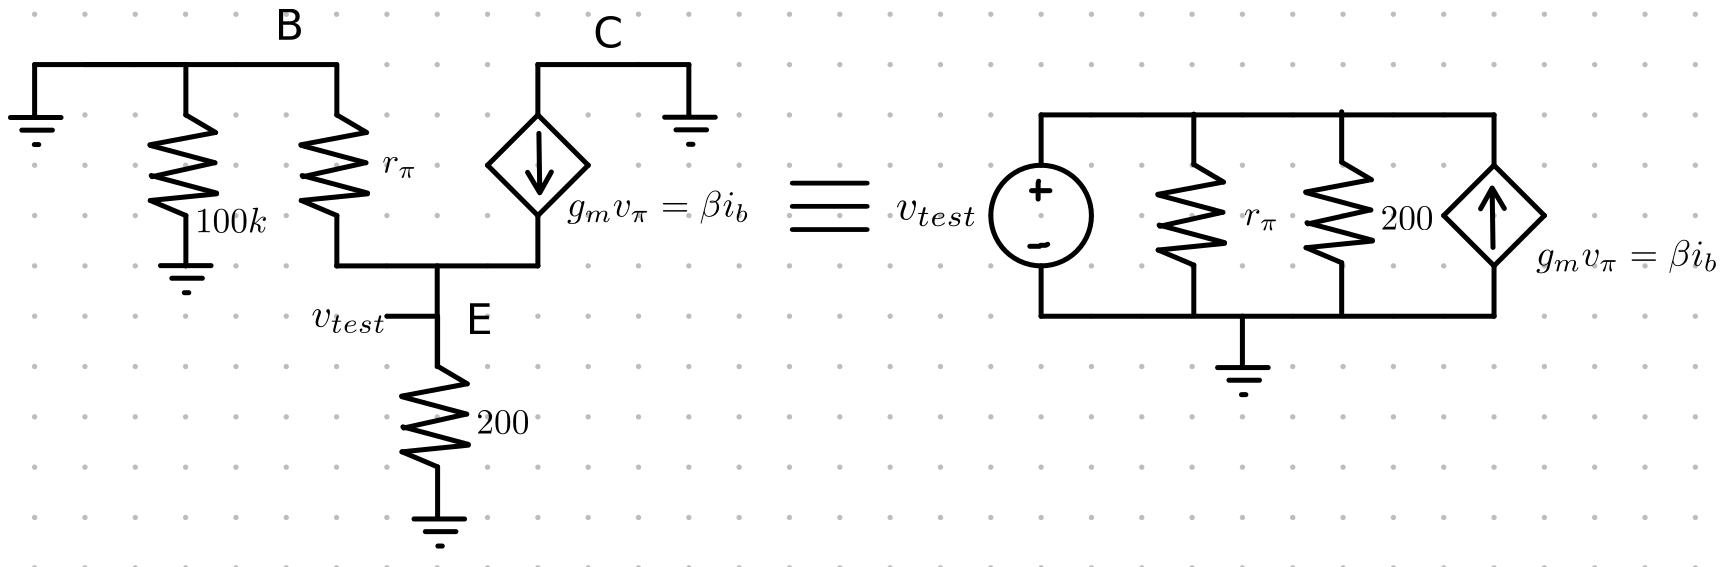
\includegraphics[width=0.7\linewidth]{bjt-ex3}
		\end{center}
		And now I can just solve for the resistance:
		\begin{align*}
			&v_{test} = v_\pi = r_\pi i_B\\
			&i_{test} = \beta i_B + i_B + \frac{v_\pi}{200} = \beta i_B + i_B + \frac{r_\pi i_B}{200}\\
			&R_{test} = R_{out} = \frac{v_{test}}{i_{test}} = \frac{r_\pi i_B}{\beta i_B + i_B + \frac{r_\pi i_B}{200}} = \frac{r_\pi}{\beta + 1 + \frac{r_\pi }{200}} = 15.4
		\end{align*}
		
	\end{mdframed}
	
	\subsection{Early Effect}
	In the real world the current has a dependance on the voltage. This is called the Early effect. To model this, we can add a \textbf{resistor} with resistance $r_0$ between the collector and base. 
	
	When dealing with the early effect, we are given a voltage valus $V_A$ which is specific to the BJT we are working with. This allows us to calculate $r_0$. 
	\begin{align*}
		r_0 = \frac{V_A}{I_C}
	\end{align*}
	Then we can just proceed with the analysis steps as normal. The analysis does get more complex, but it is the same general process. 
	
	We just need to change the models to:
	\begin{center}
		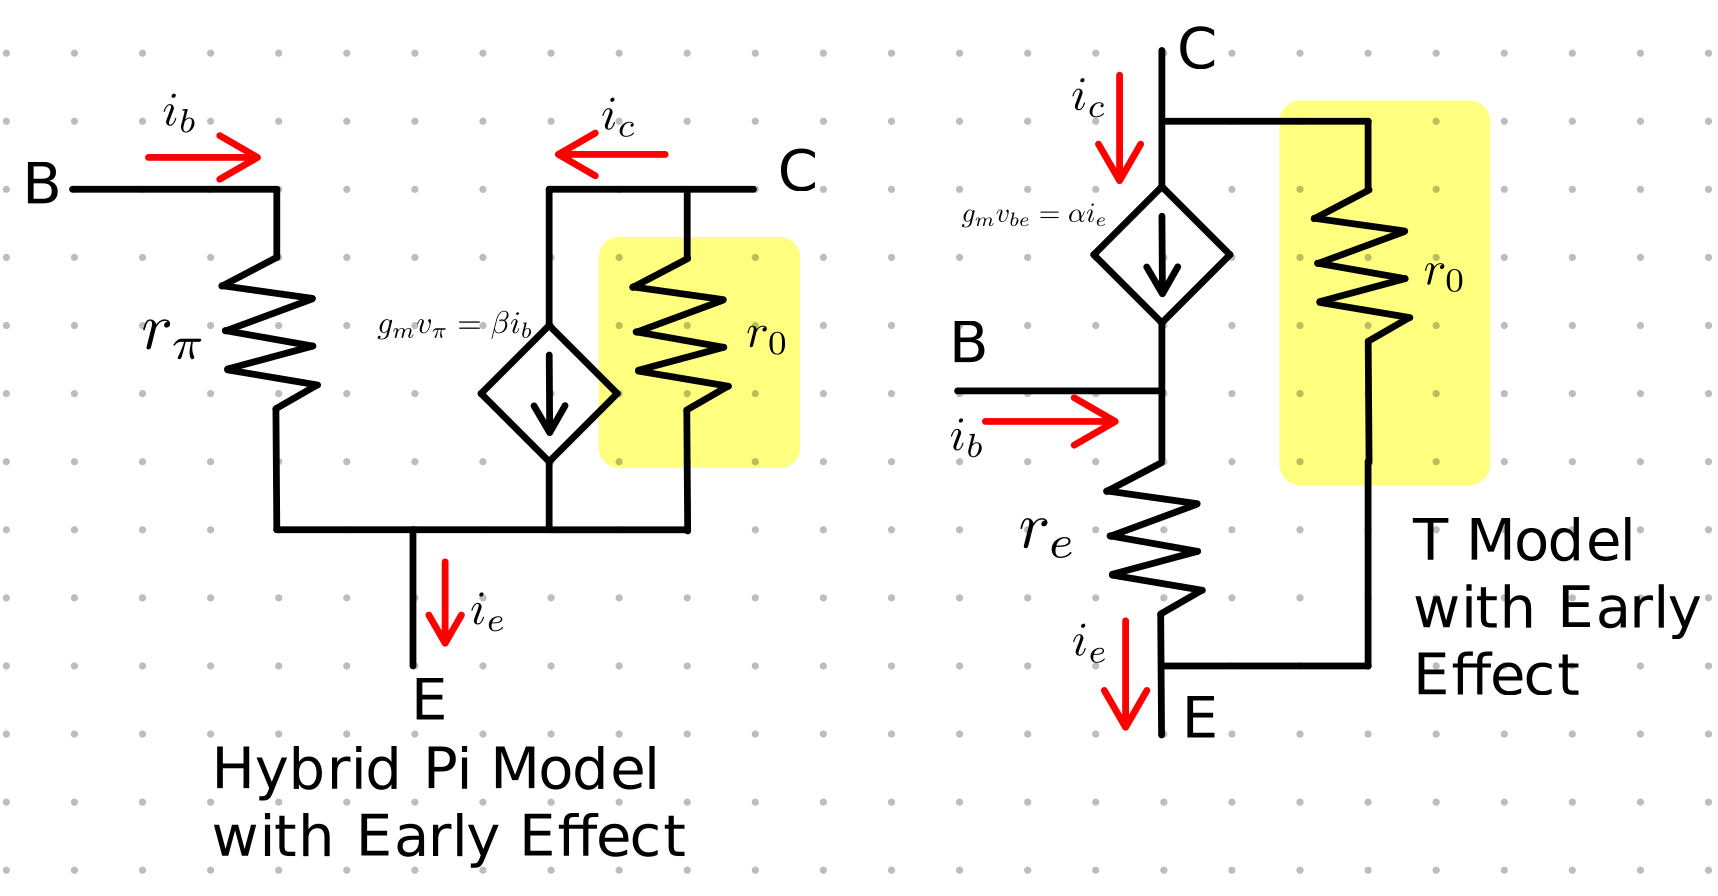
\includegraphics[width=0.8\linewidth]{hybridpi-tmodel-w-early}
	\end{center}
	
	\section{Metal Oxide Semiconductor Field Effect Transistor (MOSFET)}
	A MOSFET has 3 connections. The\textbf{ Source, Gate, and Drain}. There is \textbf{no current in the gate} since it does not directly touch the materials (therefore \textbf{source current and drain current are same}). It is just used to generate an electric field to move the charges. 
	\begin{center}
		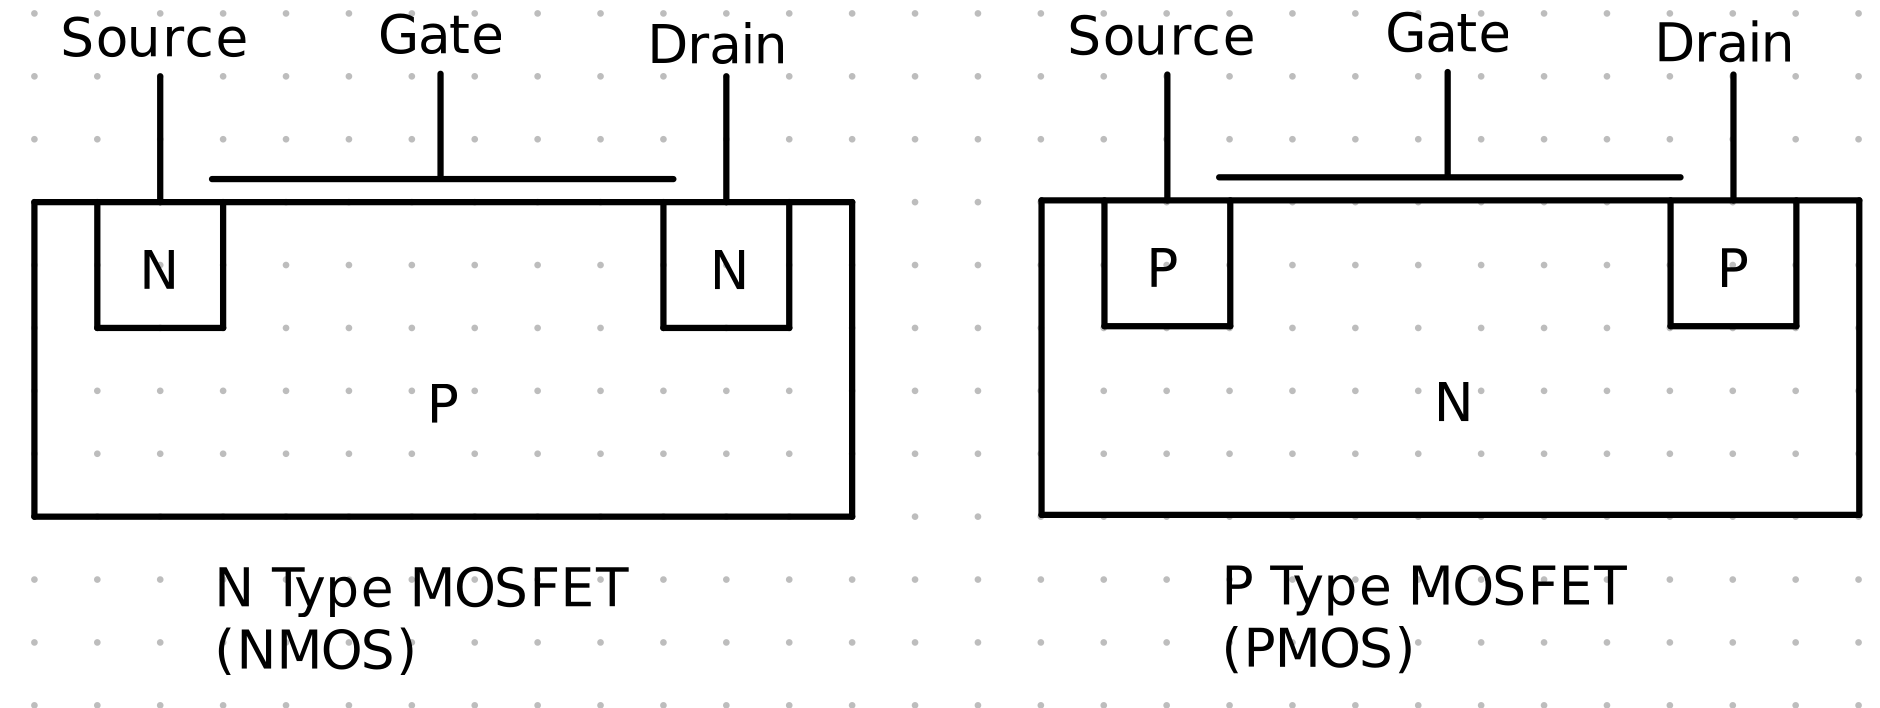
\includegraphics[width=0.8\linewidth]{nmos-pmos}
	\end{center}
	When we apply a voltage at the gate, a channel is created where the electrons will flow from the Source to the Drain (for NMOS or Drain to Source for PMOS).
	\begin{center}
		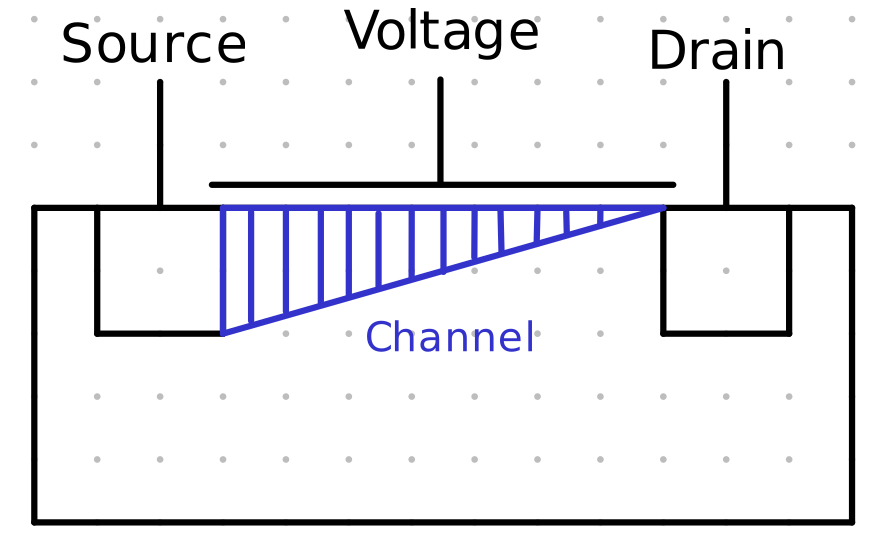
\includegraphics[width=0.35\linewidth]{mos-channel}
	\end{center}
	MOSFETs have three modes they can be in:
	\begin{itemize}
		\item Cutoff (No current)
		\item Saturation (Constant current)
		\item Triode (Changing current)
	\end{itemize}

	We have some parameters for the MOSFET. These are unique to each MOSFET and given on the datasheet.
	\begin{align*}
		&\mu C_{ox} \frac{W}{L} &V_t
	\end{align*}
	For NMOS, $V_t > 0$, and for PMOS, $V_t<0$.
	
	The symbols are:
	\begin{center}
		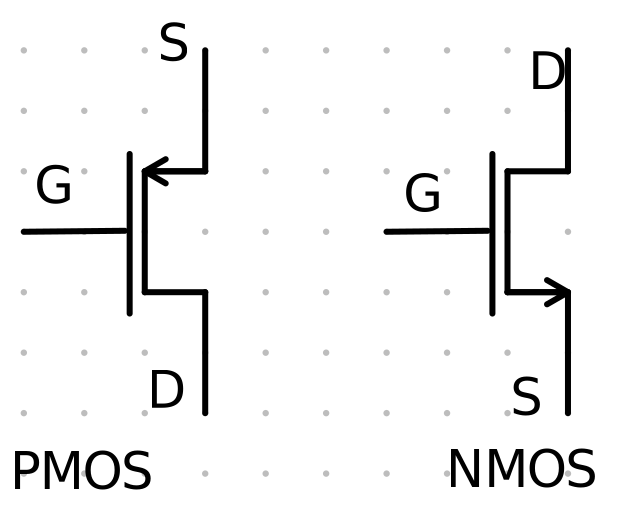
\includegraphics[width=0.25\linewidth]{pmos-nmos-symbols}
	\end{center}
	
	
	\subsection{DC Analysis}
	To do the DC analysis, we use the following process:
	\begin{enumerate}
		\item Test for cutoff mode (No current)
		\item \textbf{If not cutoff}, Assume Saturation or Triode mode
		\item Use the transistor current equation to get $I_D$ AKA $I_S$
		\item Do more circuit analysis if required
		\item Verify the two conditions for the assumed mode (from step 2)
		\item \textbf{If conditions are not met}, then return to step 2 and assume the other mode.
	\end{enumerate}

	The conditions and transistor current equation are different for NMOS or PMOS. They depend on $V_t$ which is also referred to as $V_TH$.
	
	\textbf{NMOS ($V_{TH}>0$)}
	\begin{align*}
		&V_{GS} < V_{TH} \qquad I_D = I_S = 0 &\text{Cutoff Conditions and Current}\\
		&V_{GS} > V_{TH} \qquad V_{DS} < V_{GS} - V_{TH} &\text{Triode Conditions}\\
		&I_D = I_S = \mu_n C_{ox} \frac{W}{L} \left((V_{GS}-V_{TH})V_{DS} - \frac{1}{2}V^2_{DS}\right)&\text{Triode Current}\\
		&V_{GS} > V_{TH} \qquad V_{DS} \ge V_{GS} - V_{TH}&\text{Saturation Conditions}\\
		&I_D = I_S = \frac{1}{2}\mu_n C_{ox} \frac{W}{L} (V_{GS} - V_{TH})^2(1+\lambda V_{DS})&\text{Saturation Current}
	\end{align*}
	\textbf{PMOS ($V_{TH}<0$)}
	\begin{align*}
		&V_{GS} > V_{TH} \qquad I_D = I_S = 0 &\text{Cutoff Conditions and Current}\\
		&V_{GS} < V_{TH} \qquad V_{DS} \ge V_{GS} - V_{TH} &\text{Triode Conditions}\\
		&I_D = I_S = \mu_p C_{ox} \frac{W}{L} \left((V_{SG}-|V_{TH}|)|V_{DS}| - \frac{1}{2}V^2_{DS}\right)&\text{Triode Current}\\
		&V_{GS} < V_{TH} \qquad V_{DS} < V_{GS} - V_{TH}&\text{Saturation Conditions}\\
		&I_D = I_S = \frac{1}{2}\mu_p C_{ox} \frac{W}{L} (V_{SG} - |V_{TH}|)^2(1+\lambda |V_{DS}|)&\text{Saturation Current}
	\end{align*}
	
	\subsection{AC Analysis}
	When we are doing the ac analysis just like the BJT we cannot have any answers with a \textbf{time dependant current or voltage}. 
	
	We often want to find the same parameters such as the voltage gain, or current gain. 
	
	We follow a similar procedure to the BJT where we first do DC analysis to find the operating mode, then we go into ac mode and sub in the ac model. Then we can find what we want to find. 
	
	The ac model is:
	\begin{center}
		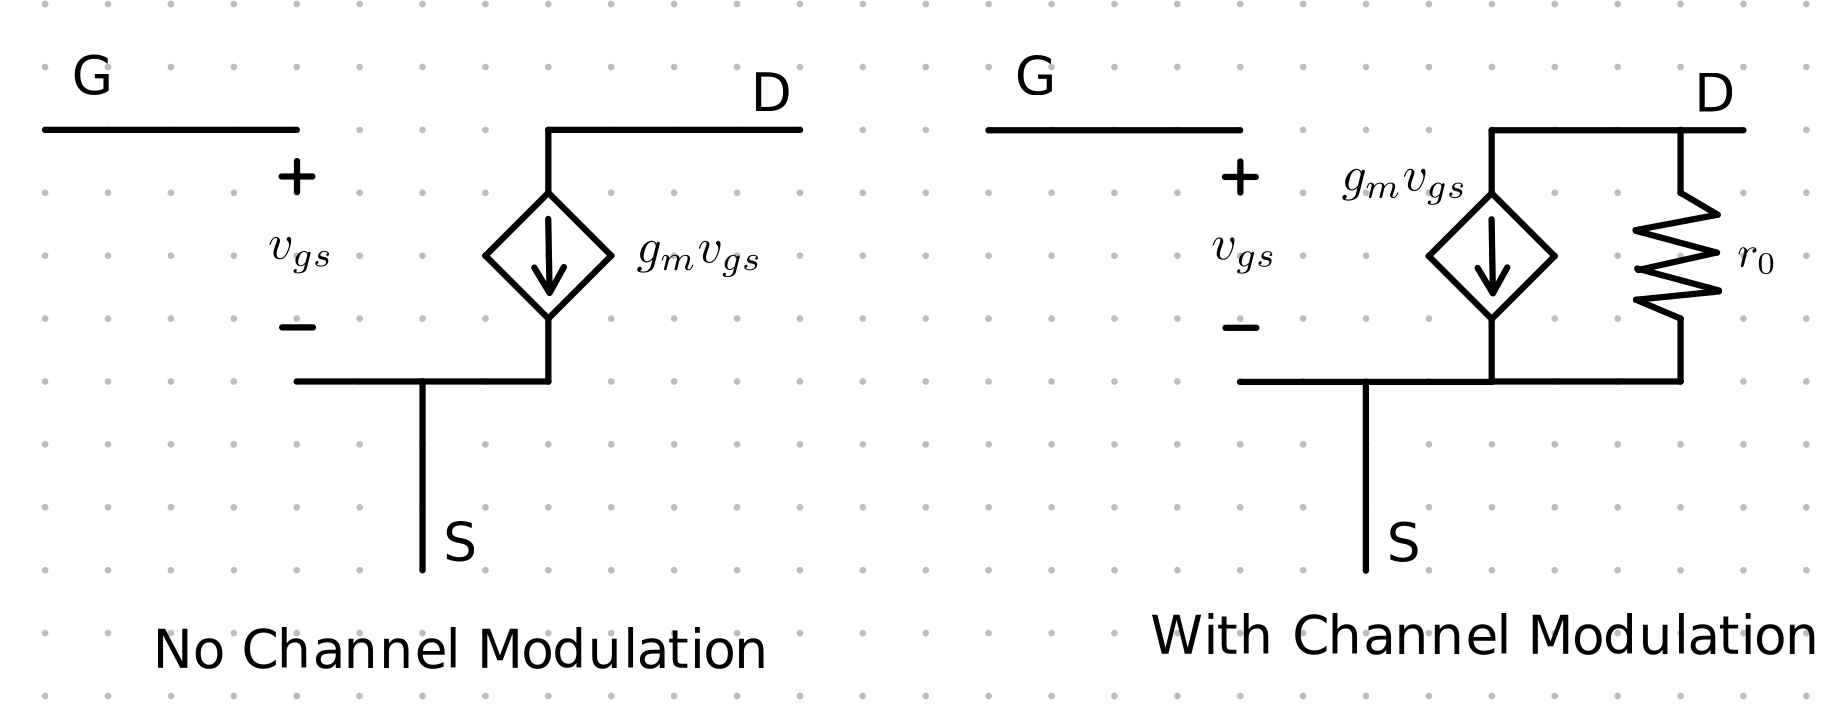
\includegraphics[width=0.8\linewidth]{mosfet-ac-model}
	\end{center}

	\subsection{Channel Modulation}
	This is the same idea of early effect for BJT but for MOSFET. 
	
	As the channel width increases, its\textbf{ resistance changes}. So we need to account for this. 
	
	We have the parameter $\frac{1}{V_A} = \lambda$.
	
	This only affects the saturation mode equation hence the term $1+\lambda V_{DS}$ at the end of those current equations. 
	
	We add a resistor $r_0$ with value of:
	\begin{align*}
		r_0 = \frac{1}{I_D \lambda}
	\end{align*}

	\begin{mdframed}
		\textbf{Ex. }We have the following NMOS circuit, find $\frac{V_o}{V_{sig}}$. Consider channel modulation. 
		\begin{center}
			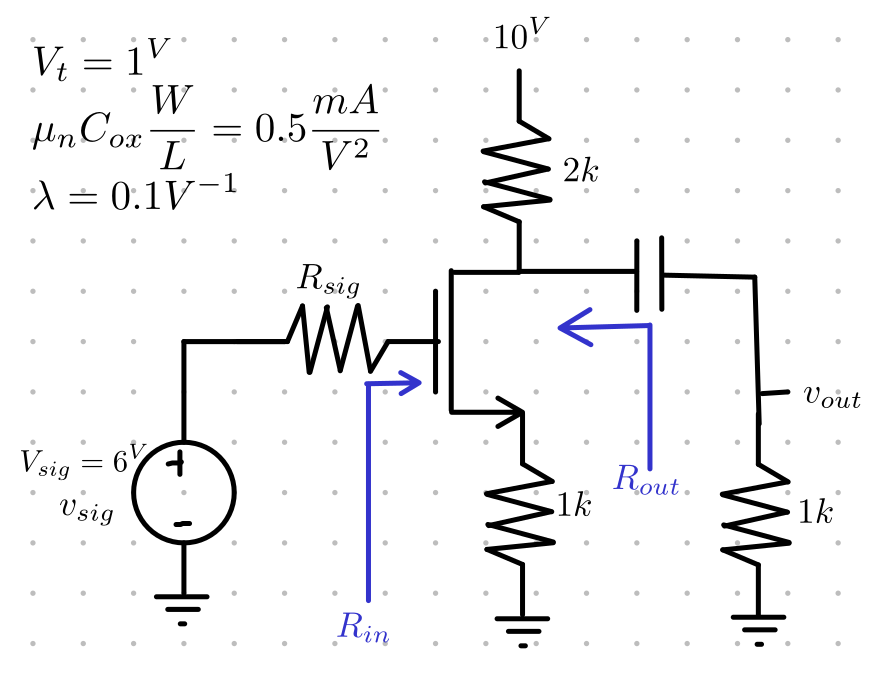
\includegraphics[width=0.4\linewidth]{mosfet-ex}
		\end{center}
		Notice how since there is never any current at the gate we can disregard $R_{sig}$ for all analysis.
		
		First we need to start with the DC analysis to see what mode it is in. I will disable the ac source, and open circuit the capacitor. Then I can test the modes. 
		
		I will test saturation mode. 
		\begin{align*}
			I_D &= \frac{1}{2}\mu_n C_{ox} \frac{W}{L} (V_{GS} - V_t)^2 = \frac{0.5}{2}(6-(1k\cdot I_D)-1)^2 = 0.25(6-I_D-1)^2 \\ &\implies I_D=2.10mA \qquad I_D=11.90mA
		\end{align*}
		Now I need to check the currents to see which one is correct. 
		\begin{align*}
			V_{GS} > V_t &\implies 6-(2.10\cdot 1) = 3.899 > 1 \qquad &\checkmark \\
			V_{DS} > V_{GS} - V_t &\implies 10-2\cdot 2.10 - 2.10= 3.697 > 3.899-1 \qquad &\checkmark
		\end{align*}
		So it must be 2.10mA since there cannot be 2 answers. Now I can find the circuit parameters:
		\begin{align*}
			&g_m = \sqrt{2\mu_n C_{ox}\frac{W}{L} I_D} = 1.449 &r_0 = \frac{1}{\lambda I_D} = 4.762k\Omega
		\end{align*}
		Now we can move to the ac model. 
		\begin{center}
			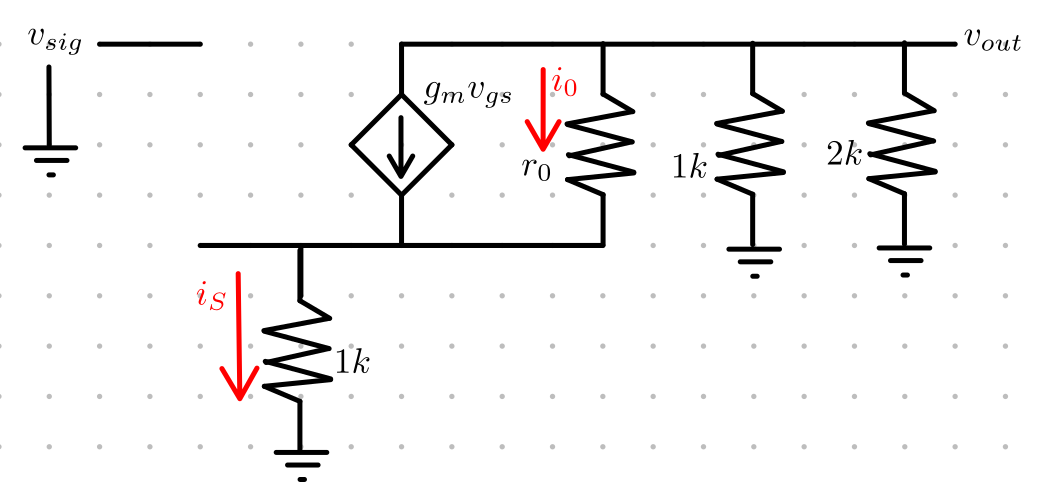
\includegraphics[width=0.5\linewidth]{mosfet-ex1}
		\end{center}
		To find the $\frac{v_o}{v_{sig}}$ I can make a lot of KVL and KCL loops/nodes, and then solve for what we want. 
		\begin{align*}
			&v_o = i_0r_0+1k i_s&\text{KVL From out going down through $r_0$}\\
			&v_o = -(i_0 + g_m v_{gs})(1k//2k)&\text{KVL From out going down right away}\\
			&v_{sig} = v_{gs} + 1k i_s&\text{KVL From in going down}\\
			&i_s = i_0 + g_m v_{gs}&\text{KCL}
		\end{align*}
		Then I can do a lot of algebra to get:
		\begin{align*}
			&v_o = -i_s(1k//2k)\\
			&v_{sig} = \frac{i_s-\frac{-i_s (1k//2k)-1ki_s}{r_0}}{g_m} + 1k i_s\\
			&\frac{v_o}{v_{sig}} = \frac{-(1k//2k)}{\frac{1-\frac{-(1k//2k)-1k}{r_0}}{g_m} + 1k} = -0.345
		\end{align*}
		If we want to find the \textbf{input resistance}, we can see that there is no current in the gate, so therefore there is infinite resistance. 
		\begin{align*}
			R = \frac{V}{I} = \lim_{I\to 0} \frac{V}{I} = \infty
		\end{align*}
		If we wanted to find the output resistance as well, we could use a similar method to finding $\frac{v_o}{v_{sig}}$ except we are finding $\frac{v_{test}}{i_{test}}$. We would create lots of KVLs and KCLs and then solve. Finally we would get a value. 
		
		
	\end{mdframed}
	
	\section{Complementary MOSFET (CMOS) Inverter}
	A CMOS is a circuit with 2 MOSFETS, one of which is a PMOS, one is an NMOS. 
	
	The Inverter is a circuit that will take a low voltage and turn it into a high voltage, and take a high voltage and turn it into a low voltage. 
	
	It is the \verb|NOT| gate.
	\begin{center}
		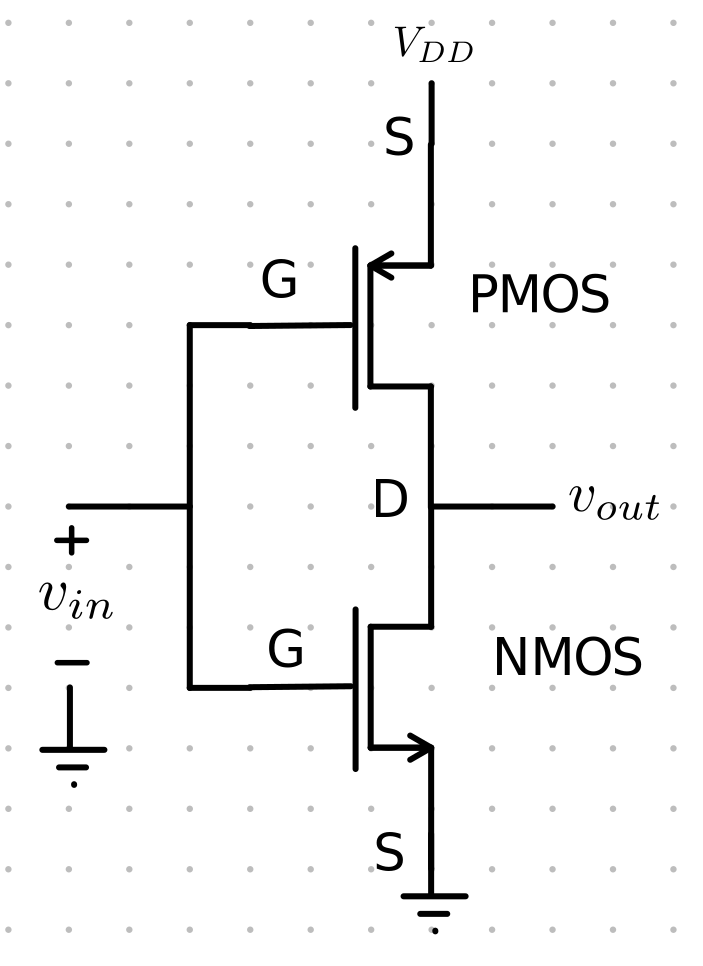
\includegraphics[width=0.34\linewidth]{cmos}
	\end{center}
	
	
	\subsection{Voltage Transfer Characteristic (VTC) of CMOS}
	\begin{center}
		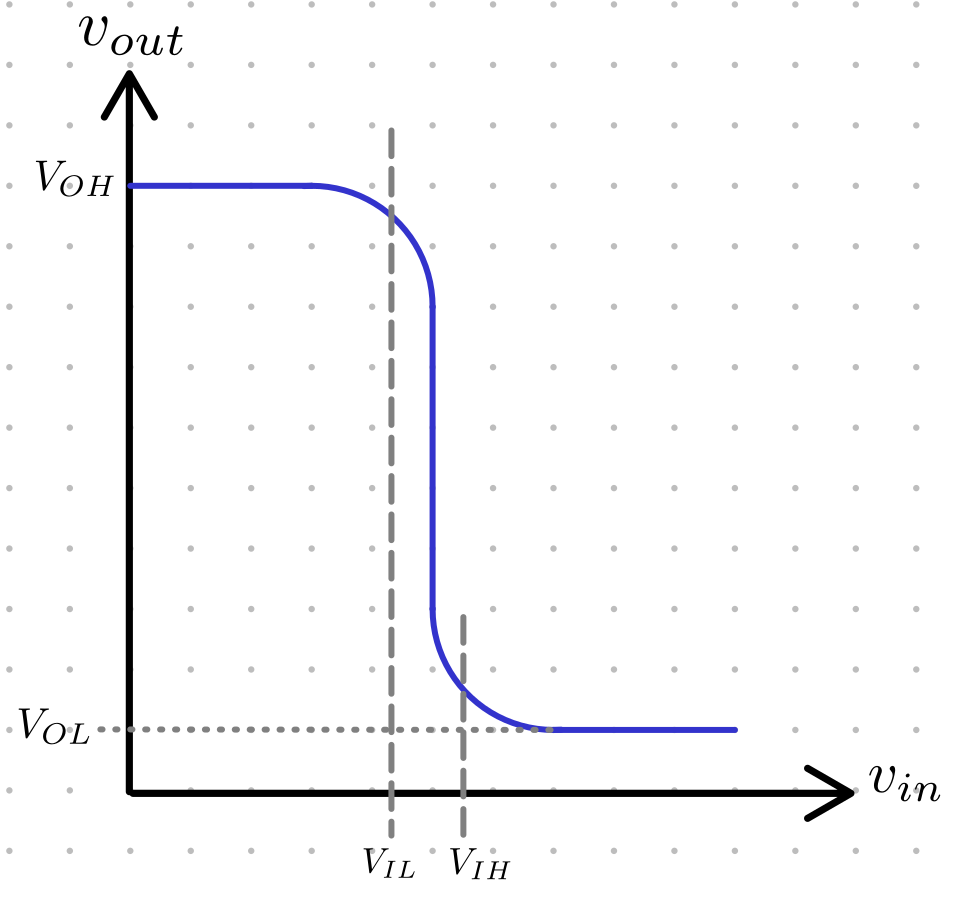
\includegraphics[width=0.4\linewidth]{CMOS-vtc}
	\end{center}
	Through the VTC, we can see that there are 5 main areas. 
	\begin{itemize}
		\item First area when $V_{out} = V_{OH}$ when the output is constant HIGH
		\item Second area where $V_{out}$ decreases, but is still HIGH
		\item Third area where $V_{out}$ is in the middle, neither HIGH or LOW (Between $V_{IL}$ and $V_{IH}$)
		\item Fourth area where $V_{out}$ is decreasing, but reached te LOW section
		\item Fifth area where $V_{out}$ is constant LOW
	\end{itemize}
	\begin{center}
		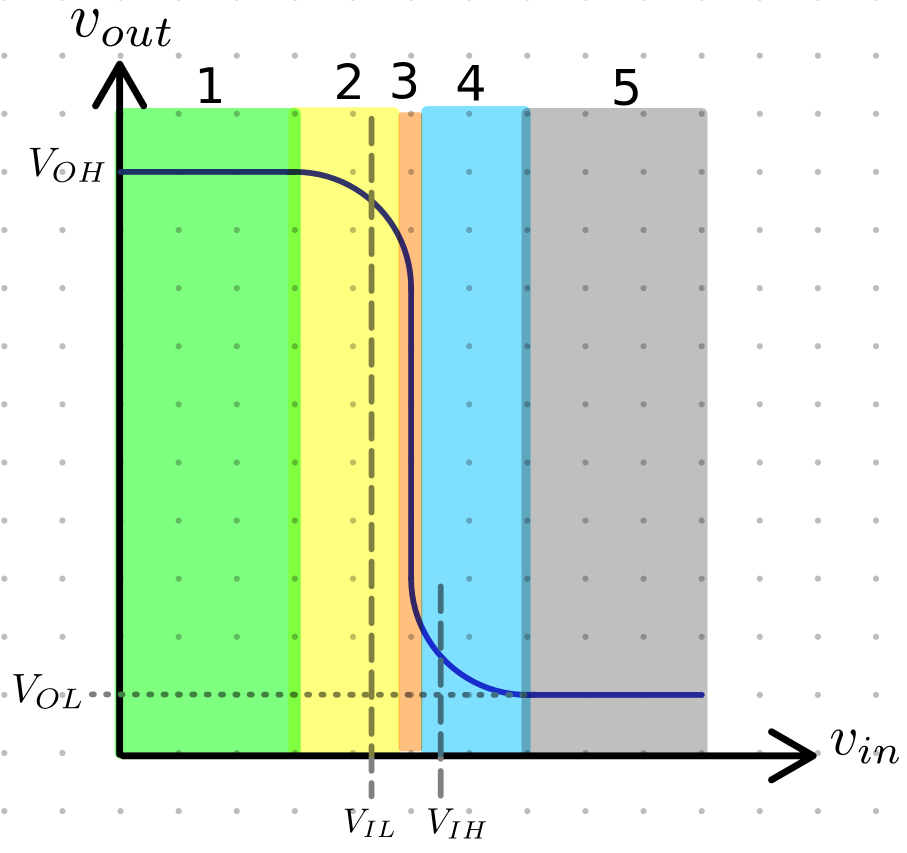
\includegraphics[width=0.4\linewidth]{CMOS-vtc-w-regions}
	\end{center}
	We can figure out through using the circuit diagram, and the MOSFET equations the states of the MOSFETs in all 5 regions:
	\begin{table}
		\centering
		\begin{tabular}{|c|c|c|}
			\hline
			Region & NMOS & PMOS \\
			\hline
			\hline
			1 & Cutoff & Triode \\
			\hline
			2 & Saturation & Triode \\
			\hline
			3 & Borderline of Triode/Saturation & Borderline of Triode/Saturation \\
			\hline
			4 & Triode & Saturation \\
			\hline
			5 & Triode & Cutoff \\
			\hline
			\end{tabular}
	\end{table}

	Most of the values are fairly straightforward to calculate, such as the main input voltage in region 3 is just half of the max input voltage $V_{DD}$. The low end of the HIGH part $V_{IL}$ and the high end of the LOW part $V_{IH}$ are:
	\begin{align*}
		&V_{IH} = \frac{1}{8} (5V_{DD} - 2V_t)  &V_{IL} = \frac{1}{8} (3V_{DD} + 2V_t)		\\
	\end{align*}

	\begin{mdframed}
		\textbf{Ex.} For the following VTC and CMOS inverter circuit, find the voltages and currents at A, B, C, ..., E. $V_{DD} = 3$, $V_{Tn} = 0.5V = -V_{Tp}$, $\mu C_{ox}\frac{W}{L} = 22222\mu A$
		\begin{center}
			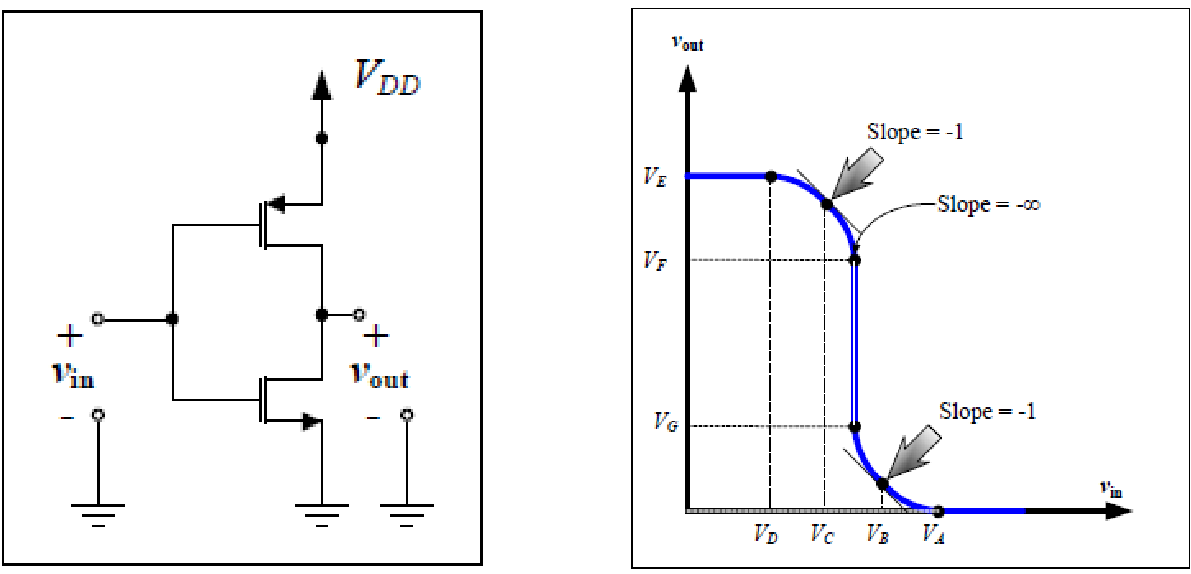
\includegraphics[width=0.8\linewidth]{cmos-ex}
		\end{center}
		If we start with $V_E$, we say that the input is 0V and the current is 0A since the NMOS is in cutoff mode. 
		
		Therefore there cannot be a voltage drop so the drain voltage is also 3V. 
		
		Then onto $V_D$. Here the input voltage must such that the NMOS almost is exiting cutoff mode. So $V_{GS} = V_{TH} = 0.5$. Therefore the current is still 0A and the drain voltage is also 0.5.
		
		To find $V_C$ and $V_B$, we can use the equations for $V_{IL}, V_{IH}$. We get 1.25 and 1.75 V. 
		
		Then to get the current for C we will use the saturation mode equation for the NMOS. We could technically use the triode mode equation for the PMOS, but we do not know the drain voltage. So it would not work. For B we use the saturation mode equation for PMOS.
		\begin{align*}
			I_S = \frac{1}{2}\mu_n C_{ox} \frac{W}{L} (V_{GS} - V_{TH})^2(1+\lambda V_{DS}) = 0.5\cdot 22.222(1.25-0 - 0.5)^2 = 6.25mA\\
			I_S = \frac{1}{2}\mu_n C_{ox} \frac{W}{L} (V_{SG} - |V_{TH}|)^2(1+\lambda V_{DS}) = 0.5\cdot 22.222(3-1.75 - 0.5)^2 = 6.25mA
		\end{align*}
		Here the input is $\frac{V_{DD}}{2}$.
		
		I can let the 2 currents equal to each other since I know that in the previous mode the NMOS is in saturation and the PMOS is in triode mode to get:
		\begin{align*}
			\frac{1}{2}\mu_n C_{ox}\frac{W}{L}_n (V_{GS} - V_t)^2 &= \mu_p C_{ox} \frac{W}{L}_p \left((V_{SG} - |V_t|)|V_{DS}|-\frac{1}{2}V_{DS}^2\right)\\
			\frac{1}{2}(\frac{V_{DD}}{2} - V_t)^2&=\left((3-\frac{V_{DD}}{2} - V_t)(3-V_{out})-\frac{1}{2}(3-V_{out})^2\right)\\
			&\implies V_{out} = 2^V
		\end{align*}
		Then the current can be obtained by just taking one of the sides of that equation:
		\begin{align*}
			I_D = \frac{1}{2}\mu_n C_{ox}\frac{W}{L}\left(\frac{V_{DD}}{2}-V_t\right)^2 = \frac{1}{2}\mu_n C_{ox}\frac{W}{L}\left(\frac{3}{2}-0.5\right) = 11.11^{mA}
		\end{align*}
		This is the same general procedure as the previous section. Except we start at the place where the PMOS is in saturation, and the NMOS is in triode. Work from the bottom up. 
		\begin{align*}
			\mu_n C_{ox} \frac{W}{L}_n \left((V_{GS1}-V_t)V_{DS1} - \frac{1}{2}V_{DS1}^2\right) &= \frac{1}{2}\mu_p C_{ox} \frac{W}{L}_p (V_{SG2} - V_t)^2\\
			\left((\frac{V_{DD}}{2}-0.5)V_{out} - \frac{1}{2}V_{out}^2\right) &= \frac{1}{2}(3-\frac{V_{DD}}{2}-0.5)^2\\
			&\implies V_{out} = 1^V
		\end{align*}
		
		To find the current I just need to use one half of the equation:
		\begin{align*}
			I_D = \frac{1}{2}\mu_p C_{ox} \frac{W}{L}_p (V_{SG2} - V_t)^2 = \frac{1}{2}\mu_p C_{ox} \frac{W}{L}_p (3-1.5 - 0.5)^2 = 11.11^{mA}
		\end{align*}
		Going to A, we know that the current is 0 since the PMOS is in cutoff mode. To find the voltage, we can see that the PMOS is just going from saturation mode to cutoff mode. So using the conditions:
		\begin{align*}
			V_{GS} > V_{TH} \implies V_{G}-V_{S} = V_{TH} \implies V_G - 3 = -0.5 \implies V_G = 2.5
		\end{align*}
		
		In summary, all these relationships (in below table) can be shown by analysing the boundary conditions between the different regions, and using the correct formulas.
		\begin{tabular}{|c|c|c|}
			\hline
			Voltage Name & Value (V) & Value of Corresponding Current ($I_{D1} = I_{D2}$) (mA) \\
			\hline
			$V_A$ & $2.5^V$ & $0^{mA}$ \\
			\hline
			$V_B$ & $1.75^V$ & $6.25^{mA}$ \\
			\hline
			$V_C$ & $1.25^V$ & $6.25 ^{mA}$ \\
			\hline
			$V_D$ & $0.5^V$ & $0^{mA}$ \\
			\hline
			$V_E$ & $3^V$ & $0^{mA}$ \\
			\hline
			$V_F$ & $2^V$ & $11.11^{mA}$ \\
			\hline
			$V_G$ & $1^V$ & $11.11^{mA}$ \\
			\hline
		\end{tabular}
	\end{mdframed}
	
	\subsection{Delay in the CMOS Inverter}
	In real life, the inverter does not change from HIGH to LOW, or from LOW to HIGH instantaneously. There is some delay.
	
	We define the time it takes for the inverter to go from LOW to halfway to HIGH as $t_{PLH}$ and from HIGH to halfway to LOW as $t_{PHL}$.
	
	We can see this quite obviously if we have a capacitor connected to the output voltage of the CMOS inverter. By definition, the voltage of the capacitor cannot change instantaneously. So there must be some delay. 
	\begin{center}
		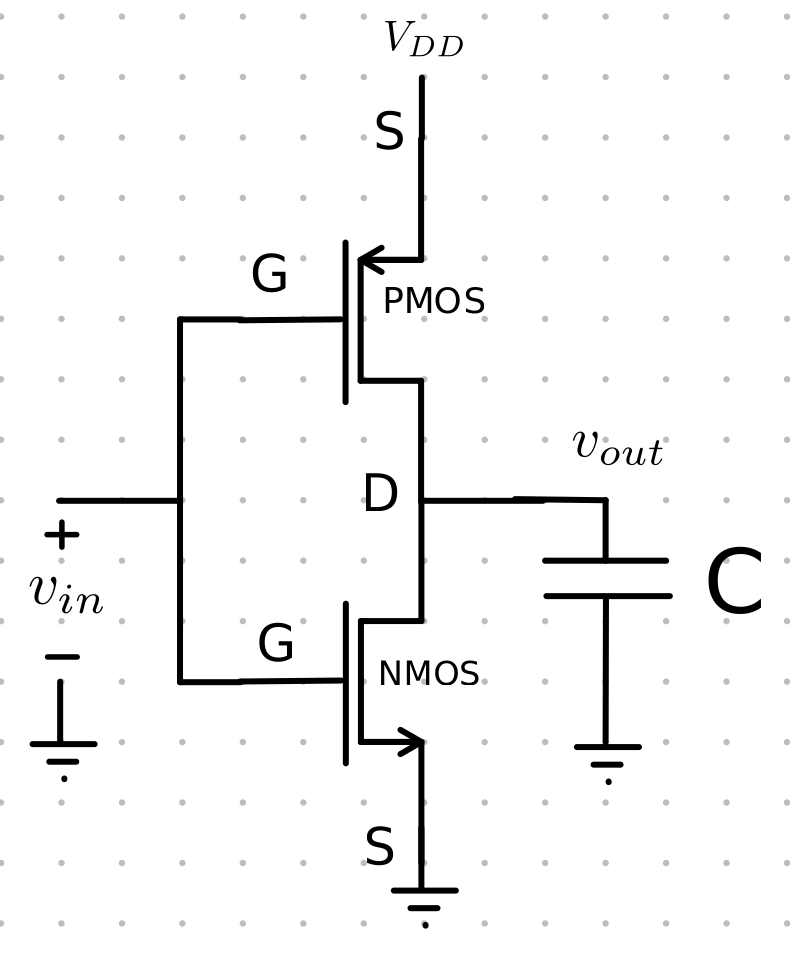
\includegraphics[width=0.4\linewidth]{not-with-cap}
	\end{center}
	We have the following equations to calculate the times given a capacitence $C$:
	\begin{align*}
		&t_{PHL} = \frac{a_n C}{\mu_n C_{ox}\left(\frac{W}{L}\right)_n V_{DD}}& \alpha_n = \frac{2}{\frac{7}{4}-\frac{3V_{tn}}{V_{DD}}+\left(\frac{V_{tn}}{V_{DD}}\right)^2}\\
		&t_{PHL} = \frac{a_p C}{\mu_p C_{ox}\left(\frac{W}{L}\right)_p V_{DD}}& \alpha_p = \frac{2}{\frac{7}{4}-\frac{3|V_{tp}|}{V_{DD}}+\left(\frac{V_{tp}}{V_{DD}}\right)^2}
	\end{align*}
	
	
	\newpage
	\section{Appendix}
	\subsection{Short Formula Sheet}
	This is just a summary of all the important formulas:
	
\textbf{Semiconductor Physics:}
	\begin{align*}
&		n_i = 5.2\times 10^{15} T^{\frac{3}{2}} e^\frac{-E_g}{2kT}\\
&		J_{drift} = q(\mu_n n+ \mu_p p) E \qquad J_{diffusion} = qD_n \frac{dn}{dx} - qD_p \frac{dp}{dx}\\
&		p_p \propto N_A \qquad n_n \propto N_D\\
&		p_pn_p = n_np_n = n_i^2\\
& 		J_{diff\_tot} = Aqn_i^2\left(\frac{D_p}{L_pN_D}+\frac{D_n}{L_nN_A}\right)\left(e^{\frac{v}{V_t}}-1\right) \text{ For PN Junction}
	\end{align*}
	\textbf{rectifier with Filter: Half wave rectifier with single ideal diode}
	\begin{align*}
		V_r &= \frac{V_p}{fRC} &\omega\Delta t = \sqrt{\frac{2V_r}{V_p}} \\
		i_{Davg} &= I_L(1+\pi\sqrt{\frac{2V_p}{V_r}}) &i_{Dmax} = I_L(1+2\pi\sqrt{\frac{2V_p}{V_r}}) 
	\end{align*}
	\textbf{Zener Diode}
	\begin{align*}
		\text{Line Regulation}=\frac{\Delta V_O}{\Delta V_s} = \frac{r_z}{r_z+R} \qquad \text{Load Regulation}=\frac{\Delta V_O}{\Delta I_L} = -\frac{r_z\times R}{r_z+R} = -r_z // R
	\end{align*}
	\textbf{BJT}
	\begin{align*}
		g_m = \frac{I_C}{V_T} \qquad r_\pi = \frac{\beta}{g_m} \qquad r_0 = \frac{V_A}{I_C} \qquad r_e = \frac{\alpha}{g_m} \qquad \alpha = \frac{\beta}{\beta+1}
	\end{align*}
	\textbf{NMOS ($V_{TH}>0$)}
	\begin{align*}
		&V_{GS} < V_{TH} \qquad I_D = I_S = 0 &\text{Cutoff}\\
		&V_{GS} > V_{TH} \qquad V_{DS} < V_{GS} - V_{TH} &\text{Triode}\\
		&I_D = I_S = \mu_n C_{ox} \frac{W}{L} \left((V_{GS}-V_{TH})V_{DS} - \frac{1}{2}V^2_{DS}\right)&\text{Triode}\\
		&V_{GS} > V_{TH} \qquad V_{DS} \ge V_{GS} - V_{TH}&\text{Saturation}\\
		&I_D = I_S = \frac{1}{2}\mu_n C_{ox} \frac{W}{L} (V_{GS} - V_{TH})^2(1+\lambda V_{DS})&\text{Saturation}
	\end{align*}
	\textbf{PMOS ($V_{TH}<0$)}
	\begin{align*}
		&V_{GS} > V_{TH} \qquad I_D = I_S = 0 &\text{Cutoff}\\
		&V_{GS} < V_{TH} \qquad V_{DS} \ge V_{GS} - V_{TH} &\text{Triode}\\
		&I_D = I_S = \mu_p C_{ox} \frac{W}{L} \left((V_{SG}-|V_{TH}|)|V_{DS}| - \frac{1}{2}V^2_{DS}\right)&\text{Triode}\\
		&V_{GS} < V_{TH} \qquad V_{DS} < V_{GS} - V_{TH}&\text{Saturation}\\
		&I_D = I_S = \frac{1}{2}\mu_p C_{ox} \frac{W}{L} (V_{SG} - |V_{TH}|)^2(1+\lambda |V_{DS}|)&\text{Saturation}
	\end{align*}
	\textbf{Small Signal Parameters for NMOS or PMOS}
	\begin{align*}
		g_m = \sqrt{2\mu C_{ox} \frac{W}{L}I_D} = \mu C_{ox} \frac{W}{L} (V_{GS} - V_TH) \qquad r_0 = \frac{1}{\lambda I_D}
	\end{align*}
	\textbf{CMOS Inverter}
	\begin{align*}
		&V_{IH} = \frac{1}{8} (5V_{DD} - 2V_t)  &V_{IL} = \frac{1}{8} (3V_{DD} + 2V_t)		\\
		&t_{PHL} = \frac{a_n C}{\mu_n C{ox}\frac{W}{L}_n V_{DD}}& \alpha_n = \frac{2}{\frac{7}{4}-\frac{3V_{tn}}{V_{DD}}+\left(\frac{V_{tn}}{V_{DD}}\right)^2}\\
		&t_{PHL} = \frac{a_p C}{\mu_p C{ox}\frac{W}{L}_p V_{DD}}& \alpha_p = \frac{2}{\frac{7}{4}-\frac{3|V_{tp}|}{V_{DD}}+\left(\frac{V_{tp}}{V_{DD}}\right)^2}
	\end{align*}
	
	
	
	
	
\end{document}